\documentclass[fr]{../../../eplsummary}

\usepackage{bm}
\usepackage{float}
\usepackage{framed}
\usepackage{graphicx}
\usepackage{pdfpages}
\usepackage{palatino}
\usepackage{enumitem}
\usetikzlibrary{arrows}

\usepackage[squaren, Gray, cdot]{SIunits} % for ohm, henries,. . .
\usepackage[bottom]{footmisc}
\usepackage{desclist}
\usepackage{tocloft}

\hypertitle{Introduction aux télécommunications}{6}{ELEC}{1930}
{Syméon Malengreau\and Nicolas Houtain\and Nicolas Kabasele \and Florian
Thuin}
{Jérôme Louveaux}

\section{Introduction}

\begin{description}
	\item[Télécommunications] Transmission d'information sous la forme de signaux électriques, sur un canal de communication
\end{description}

\subsection{Canaux de communications}

Deux types de canaux de communications: \textit{filaires} (ligne
téléphonique, cable coaxial,\ldots) et \textit{sans fils} (ondes
électromagnétiques. Trois éléments caractérisent ces canaux:
\begin{description}
\item[L' Atténuation] (ou affaiblissement) est la diminution de l'amplitude ou de la puissance d'une onde ou d'un signal lors de sa transmission~\cite{AttWiki}. Il augmente avec la distance.
\item[Le Bruit] est une partie du signal transmis dont on ne peut pas tirer d'information~\cite{BruitWiki}.
\item[La Distorsion] ou \textbf{dispersion} est l'ensemble des modifications indésirables d'un signal~\cite{DistWiki}.
\end{description}

Il existe deux moyens de représenter les informations par des signaux:
\begin{itemize}
\item Signaux analogiques
\item Signaux numériques (valeurs binaires)
\end{itemize}

Une troisième technique est la \textbf{numérisation} qui est la
transformation de signaux analogiques en signaux numériques.

\begin{figure}[H]
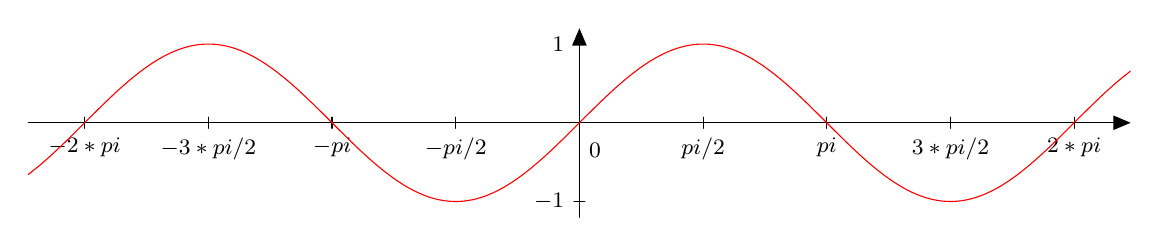
\begin{tikzpicture}[line cap=round,line join=round,>=triangle 45,x=1.0cm,y=1.0cm]
\draw[->,color=black] (-7,0) -- (7,0);
\foreach \x in {-2*pi, -3*pi/2, -pi, -pi/2, pi/2, pi, 3*pi/2, 2*pi}
\draw[shift={(\x,0)},color=black] (0pt,2pt) -- (0pt,-2pt) node[below] {\footnotesize $\x$};
\draw[->,color=black] (0,-1.2) -- (0,1.2);
\foreach \y in {-1,1}
\draw[shift={(0,\y)},color=black] (2pt,0pt) -- (-2pt,0pt) node[left] {\footnotesize $\y$};
\draw[color=black] (0pt,-10pt) node[right] {\footnotesize $0$};
\clip(-7,-1.2) rectangle (7,1.2);
\draw[smooth,samples=100,domain=-7.0:7.0, color=red] plot(\x,{sin(((\x))*180/pi)});
\end{tikzpicture}
\caption{Représentation d'un signal sinusoïdal}
\end{figure}

\subsection{Transformée de Fourier}

La transformée de Fourier est un moyen de représenter un signal par un ensemble de fréquence.
$$f(t) \Leftrightarrow F(\omega)$$

\[ F(\omega) = \int_{-\infty}^{+\infty} f(t) e^{-j\omega t} dt \]

\[ f(t) = \frac{1}{2\pi} \int_{-\infty}^{+\infty} F(\omega) e^{j\omega
t} d\omega \]

La transformation de Fourier permet d'analyser tout signal en une somme
de sinusoïdes.

\subsection{Modulation}

\begin{description}
  \item [Note]
Les différents systèmes de télécommunications utilisent des bandes de
fréquence bien précises pour chaque tâche.
\end{description}

La modulation permet de transposer un signal autour d'une fréquence définie.
Cette technique est utilisé pour partager les différentes bandes de fréquences.

\begin{center}
  \textit{Un \textbf{signal modulé} est un \textbf{signal modulant} mis sur une \textbf{porteuse} à la fréquence désiré}
\end{center}

\begin{description}
\item[Le Multiplexage] permet de faire passer plusieurs informations sur
    un seul support de fréquence. Les différents symboles sont combinés
    grâce à un multiplexeur.
  Deux types de multiplexage: \textbf{temporel} et \textbf{fréquentiel}.
\end{description}

\subsection{Exemples: radio et télévision}

\subsubsection{Radio}

Avec la radio les sons gauche (G) et droit (D) sont envoyés ensemble sous un
signal $S_1 = G+D$ de façon à ce que les radios mono puissent le
recevoir et un autre signal est envoyé pour le stéréo $S_2 = G-D$. Le
signal stéréo peut être recréé par l'opération suivante:
\begin{eqnarray*}
G &=& S_1 + S_2\\
D &=& S_1 - S_2
\end{eqnarray*}

\subsubsection{Télévision}

Pour la télévision le procédé est assez différent, la luminance (niveau
de gris) des lignes est envoyée avec une pulsation de synchronisation (\textbf{synchronizing pulse}) entre chaque ligne.

Aussi pour rendre les images fluides pour la vue humaine on entrelace
les lignes, c'est-à-dire que l'on envoie d'abord la moitié des lignes
(une ligne sur deux), et puis on envoie les lignes qui reste (\textbf{1 image = 2 trames}).

Pour l'envoi des couleurs, l'idée est la même qu'avec la radio, on va
garder l'envoi de la luminance pour que les vieilles télévision puissent
toujours lire l'image et l'on va rajouter d'autres signaux pour pouvoir avoir la couleur.
Soient $RGB$ les couleurs (red, green, blue) et $YUV$ les signaux (luminance Y et chrominance U V).
\begin{eqnarray*}
Y &=& 0.3R + 0.59G + 0.11B\\
U &=& 0.493 (B-Y)\\
V &=& 0.877 (R-Y)
\end{eqnarray*}
De nos jours la télévision numérique a remplacé la télévision analogique
et les images sont désormais envoyées en contenu binaire.

\subsection{Numérisation}

La \textbf{numérisation} va permettre de passer d'un signal analogique à
un signal numérique. On va pour cela \textbf{échantillonner} le signal
(capturer des valeurs à intervalle fixe). Les avantages des signaux numériques sont:
\begin{itemize}
\item le traitement et stockage de l'information;
\item la régénération du signal par des codes correcteurs et détecteurs d'erreur.
\end{itemize}

Un signal analogique est représenté par des valeurs continues (ensemble
$\mathbb{R}$) alors qu'un signal numérique est représenté par des valeurs
discrètes (ensemble des chiffres représentables par des séries de 0 et
de 1). Le procédé de transformation est appelé \textbf{quantification}
lors duquel on remplace les valeurs continues reçues par les valeurs
discrètes qui s'en rapprochent le plus. \newline

Il faut faire très attention lors de l'échantillonnage des erreurs
possibles. En effet, choisir un intervalle de temps trop large pour capturer les valeurs peut causer des erreurs. (On interpretera un signal d'une manière différente).

\begin{description}
\item[Théorème de Shannon] La fréquence d'échantillonage doit être au moins 2 fois la fréquence maximum du signal
\end{description}

\begin{figure}[H]
    \begin{center}
        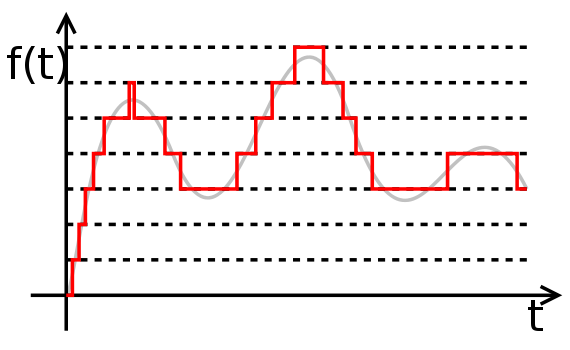
\includegraphics[width=0.5\linewidth]{img/quantification_signal.png}
        \caption{Quantification (en rouge) d'un signal continu (en
        gris)}
    \end{center}
\end{figure}

\newpage
\section{Lignes}

\subsection{Caractérisation des lignes}

Trois éléments caractérisent une ligne: 
\begin{enumerate}
    \item L'atténuation
    \item La distorsion
    \item Le bruit
\end{enumerate}

Tous ces éléments dépendent de la géométrie, des matériaux et des
conditions dans lesquelles ces lignes opèrent. Il y a de nombreux types de lignes différents:
\begin{itemize}
	\item Ligne bifilaire
	\item Ligne coaxiale
	\item Ligne unifilaire
	\item Ligne à ruban
	\item Fibre optique
	\item ...
\end{itemize}

\subsection{Modélisation d'une ligne}
On représente habituellement les lignes comme une résistance $R'$
($\ohm$/m), une conductance $G'$, une inductance $L'$ et une capacité $C'$. Le morceau de ligne suivant se répète tout au long de la ligne:
\begin{figure}[H]
\centering
\begin{picture}(280,110)
	%\put(0,0){\framebox(280,140)}
	\put(10,10){\line(1,0){260}}
	\put(10,100){\line(1,0){60}}
	\put(10,100){\vector(1,0){30}}
	% Resistance
	\put(70,95){\framebox(30,10)}
	\put(100,100){\line(1,0){25}}
	% Inductance
	\put(125,100){\line(1,2){5}}
	\put(130,110){\line(0,-1){20}}
	\put(130,90){\line(1,2){10}}
	\put(140,110){\line(0,-1){20}}
	\put(140,90){\line(1,2){10}}
	\put(150,110){\line(0,-1){20}}
	\put(150,90){\line(1,2){5}}
	\put(155,100){\line(1,0){115}}
	\put(200,100){\vector(1,0){50}}
	% Capacite
	\put(175,100){\line(0,-1){42}}
	\put(175,52){\line(0,-1){42}}
	\put(165,58){\line(1,0){20}}
	\put(165,52){\line(1,0){20}}
	% Conductance
	\put(220,100){\line(0,-1){30}}
	\put(220,40){\line(0,-1){30}}
	\put(215,40){\framebox(10,30)}
	% Vecteurs
	\put(10,80){\vector(0,-1){50}}
	\put(270,80){\vector(0,-1){50}}
	% Texte
	\put(80,80){$R'$}
	\put(135,80){$L'$}
	\put(150,45){$C'$}
	\put(200,45){$G'$}
\end{picture}
\caption{Modélisation d'une ligne}
\end{figure}

Ces paramètres varient suivant le type de ligne, fréquence et matériel
utilisé. L'équation des télégraphistes nous donne la relation suivante (avec $z$ la position, $t$ le temps et $v$ la tension sur la ligne):
$$\frac{\partial^2 v}{\partial z^2} = LC \frac{\partial^2 v}{\partial t^2} + (RC + LG)\frac{\partial v}{\partial t}+RGv$$

Dans le cas d'un contexte où les pertes seraient négligeables ($R=G=0$) nous obtiendrons la formule suivante.
$$\frac{\partial^2v}{\partial z^2}=LC\frac{\partial^2v}{\partial t^2}$$

Qui fait le lien entre une variation de tension en fonction de la position et une variation de la tension en fonction du temps. Posons $c = \frac{1}{\sqrt{LC}}$ et nous avons la tension:
$$v = f(z+ct) + g(z-ct)$$

Il s'agit en fait de l'expression de la tension en fonction d'un courant dans un sens $f$ et de sa réflexion dans l'autre sens $g$.

\subsection{Effet pélliculaire}

\begin{description}
  \item[L'effet pélliculaire] (ou l'effet de peau) est un effet électromagnétique qui repousse les lignes de courant vers la surface du conducteur. Les électrons vont s'amasser sur les bords. ~\cite{B31}
\end{description}

Cet effet de peau va en fait diminuer la surface de la ligne qui est
effectivement parcourue par du courant et donc augmenter la résistance de celui-ci comme $\sqrt{f}$. Il est causé par la création d'un champ magnétique.
$$\nearrow \mathrm{fréquence} \Rightarrow \nearrow \mathrm{effet\ de\
peau} \Rightarrow \nearrow \mathrm{résistance}
\Rightarrow  \nearrow \mathrm{pertes}$$

\subsection{Atténuation}
\begin{description}
  \item[L'atténuation d'un signal] d'une ligne peut être calculé comme
      étant $10 log(P_1/P_2)$, avec $P_1$ la puissance d'entrée et $P_2$
      la puissance de sortie. Cette atténuation se mesure en
      \textbf{décibels} ($dB$).
\end{description}

L'atténuation comme rapport de puissances s'exprime $10
log(\frac{P1}{P2})$ en décibels.

On sait que $P = \frac{V^{2}}{R}$, donc $\frac{p_{1}}{p_{2}} =
\frac{v_{1}^{2}}{v_{2}^{2}}$. Si on souhaite exprimer l'équation de
l'atténuation sous forme de tensions, on a :
\[ 10log\frac{p_{1}}{p_{2}} = 10log\frac{v_{1}^{2}}{v_{2}^{2}} =
20log\frac{v_{1}}{v_{2}} \]

\subsection{Dispersion}

Soient le nombre de pulsation $\omega = 2\pi f$, le vecteur d'onde $\beta = \frac{2\pi}{\lambda}$ et $\lambda$ la longueur d'onde, on a la \textbf{vitesse de phase}:
$$v_{ph}=\frac{\omega}{\beta}$$

La dispersion d'un signal provient des différentes vitesses de déplacement des fréquences constituant une onde. L'onde à tendance à s'étaler sur le temps plus la ligne sera longue.

\subsection{Impédance caractéristique}

\begin{description}
  \item[La loi d'Ohm] caractérise une tension $v$ en fonction d'une résistance $r$ (ou $z$ pour les résistances avec des nombres complexes) et d'un courant $i$:
    $$v = ri  \textrm{ ou } v = zi$$
\end{description}

 $z$ est totalement réel pour une résistance pure et totalement imaginaire pour une inductance/capacité pure.

  \paragraph{}
Nous allons maintenant parler de l'impédance d'une ligne en fonction de son impédance d'entrée $Z_{in}$.
\begin{itemize}
\item Dans le cas d'une \textbf{ligne infinie} l'impédance d'entrée est égale à l'impédance caractéristique de la ligne $Z_{in} = Z_c$
\item Si une ligne se termine sur une impédance $Z_c$ alors si cette ligne est \textbf{adaptée} elle ne présentera pas de réflexions et $Z_{in} = Z_c$
\end{itemize}
On peut calculer cette impédance caractéristique, le cas dans lequel la ligne serait adaptée:
$$Z_c = \sqrt{\frac{R+j\omega L}{G+ j\omega C}}$$
Dans le cas où les pertes seraint nulles nous aurions:
$$Z_c = \sqrt{\frac{j\omega L}{j\omega C}} = \sqrt{\frac{L}{C}}$$

\subsection{Exposant de propagation}

Maintenant il arrive qu'il y ait de la dispersion (\textit{déphasage}) et de l'affaiblissement linéique (\textit{atténuation}). Soient $\alpha$ l'\textbf{atténuation} et $\beta$\footnote{C'est le même beta que dans la partie sur la dispersion ci-dessus} le \textbf{déphasage}, nous calculons \textbf{l'exposant de propagation} $\gamma$:
$$\gamma = \sqrt{(R + j\omega L)(G + j\omega C)} = \alpha + j\beta$$
Habituellement dans une ligne $G$ est négligeable, deux cas se présentent à nous~\cite{Propagation}:

\subsubsection{Cas $\omega L << R$}
Ce cas correspond au cas où le fil a beaucoup de résistance. \newline

\textbf{L'exposant de propagation} en considérant $G$ et $\omega L$ nuls,
car ils sont négligable au vu des hypothèses de ce cas, devient :
\begin{eqnarray*}
\gamma &=& \sqrt{(R + j\omega L)(G + j\omega C)}\\
&\simeq& \sqrt{(R + j\omega L)(j\omega C)}\\
&\simeq& \sqrt{j\omega RC}\\
&\simeq& \sqrt{\frac{\omega RC}{2}} + j \sqrt{{\frac{\omega RC}{2}}}
\end{eqnarray*}

\textbf{L'impédance caractéristique} en considérant $G$ et $\omega L$ nuls devient :
\begin{eqnarray*}
Z_c &=& \sqrt{\frac{R + j\omega L}{G + j\omega C}}\\
&\simeq& \sqrt{\frac{R}{j \omega C}}
\end{eqnarray*}
On a donc $\alpha$ et $\beta$ qui sont proportionels à $\sqrt{\omega}$
et l'impédance caractéristique $Z_c$ est complexe et proportionnelle à $\frac{1}{\sqrt{\omega}}$. Il s'agit donc d'une mauvaise situation dans laquelle nous avons de la \textbf{distorsion}.

\subsubsection{Cas $\omega L >> R$}
Ce cas correspond au cas où le fil a peu de résistance. \newline

\textbf{L'exposant de propagation} en considérant $G$,
car il est négligable devient :

On a le droit lors du passage de la ligne 5 à la ligne 6 de mettre la
racine au carré car on ne s'intéresse qu'aux relations entre les variables. (\textit{Je comprends pas pourquoi à la ligne 6 un 2 apparait})

\begin{eqnarray*}
\gamma &=& \sqrt{(R + j\omega L)(G + j\omega C)}\\
&\simeq& \sqrt{(R + j\omega L)(j\omega C)}\\
&\simeq& \sqrt{-\omega^2 LC + j\omega RC}\\
&\simeq& \sqrt{j^2\omega^2 LC - j^3\omega RC}\\
&\simeq& j\omega\sqrt{LC}\sqrt{1-j\frac{R}{\omega L}}\\
&\simeq& j\omega\sqrt{LC}(1-j\frac{R}{2 \omega L})\\
&\simeq& \frac{\sqrt{LC}R}{2L} + j\omega\sqrt{LC}\\
&\simeq& \frac{R}{2}\sqrt{\frac{C}{L}} + j\omega\sqrt{LC}
\end{eqnarray*}

\textbf{L'impédance caractéristique} en annulant $G$ et $R$
\begin{eqnarray*}
Z_c &=& \sqrt{\frac{R + j\omega L}{G + j\omega C}}\\
&\simeq& \sqrt{\frac{L}{C}}
\end{eqnarray*}

Nous avons donc $alpha$ qui est indépendant de $\omega$ et $\beta$ proportionnel à $\omega$. A cela s'ajoute $Z_c$ qui est réel et indépendant de $\omega$.

\subsection{Pupinisation}

Pour le cas de lignes tel que $\omega L << R$, nous allons procéder à une \textbf{pupinisation}.
Cela consiste à insérer des inductances le long de la ligne afin d'augmenter artificiellement $L$.
Grâce à cela nous allons avoir une réduction de l'atténuation le long de la ligne.

Toutefois, la pupinisation n'est bénéfique que pour une certaine bande de fréquences car
elle cause l'atténuation des fréquences supérieures.
Puisque l'on a besoin de ces fréquences de nos jours, notamment pour l’ADSL, la pupinisation n’est donc plus utilisée\cite{resume}.

\subsection{Lignes bifilaires}

Les lignes bifilaire sont des lignes de transmission constituées de \textbf{deux fils parallèles} séparés par un \textbf{isolant}~\cite{Biwi}. Elles sont souvent rassemblées dans des quartes torsadées (quatre fils ensemble) ou encore dans des bottes de quartes (50 fils). Il arrive par contre dans ce genre de groupements que nous trouvions de la diaphonie.
\begin{description}
	\item[La diaphonie] (parfois \textit{bruit} ou \textit{crosstalk} en anglais) est l'interférence d'un premier signal avec un autre~\cite{Diwi}.
\end{description}
Avantages et inconvénients des lignes bifilaires:
\begin{itemize}
	\item[+] Faible coût
	\item[+] Connexions aisées
	\item[+] Pré-installation dans les bâtiments
	\item[+] Faible atténuation aux basses fréquences
	\item[-] Atténuation importante aux hautes fréquences
	\item[-] Rayonnement important (sensibilité aux interférences)
\end{itemize}

\subsection{Câble coaxial}

Un câble coaxial est constitué d'une \textbf{partie centrale}
(\textit{fil de cuivre}) enveloppé dans un \textbf{isolant}, puis d'un
\textbf{blindage métallique} tressé et enfin d'une \textbf{gaine
extérieure}~\cite{Coax}. Il est utilisé comme câble pour la transmission de la télédistribution.

Avantages et inconvénients du cable coaxial :
\begin{itemize}
	\item[+] Large bande passante ($\sim 500 MHz$)
	\item[+] Protection contre les interférences
	\item[+] Technique éprouvée et répandue
	\item[+] Facilité de réparation et de connexion
	\item[-] Fréquences limitées
	\item[-] Blindage jamais parfait
\end{itemize}

\subsection{Fibre optique}

Une fibre optique est un conducteur de lumière en \textbf{fil en verre ou en plastique} très fin utilisé pour la transmission de données (sous forme de lumière).~\cite{Fopt}.
\begin{description}
\item[Un mode] est un chemin emprunté par la lumière par rapport à sa réflexion et réfraction
  au sein de la fibre optique.
\item[Dispersion intermodale] phénomène correspondant à l'existence de différentes vitesses possibles pour la propagation des ondes. La distance parcourue par certains modes est différentes de celle d'autre mode.. il y a donc une dispersion du signal.~\cite{Dmod}.
\item[Transducteur]  dispositif convertissant un signal physique en un autre, par exemple un signal lumineux~\cite{Transducteur}.
\end{description}
On peut utiliser trois types de source lumineuse pour envoyer le signal lumineux, une diode LED, une diode laser ou une diode infrarouge. Voici les différents avantages et inconvénients de la fibre optique:
\begin{itemize}
	\item[+] Enorme bande passante
	\item[+] Très faible atténuation
	\item[+] Immunité à l'égard des rayonnements
	\item[+] Isolation électrique
	\item[+] Encombrement, poids, coût faibles
	\item[-] Connexions difficiles
	\item[-] Réparations difficiles
	\item[-] Disponibilité de transducteurs
	\item[-] Technologie en développement
\end{itemize}

\subsubsection{Trois manière de gérer les modes}

\paragraph{Fibre multimode à saut d'indice}

Les rayons réfléchissent plusieurs fois sur les parois de la fibre et avec une multitude d'angle différents. Le saut d'indice engendre des angles très fluctuant! Il existe donc de la dispersion intermodale.

\paragraph{Fibre multimode à gradient d'indice}

On va faire varier l'indice de réfraction plus l'on s'approchera des
parois afin que les différents faisceaux lumineux convergent vers le
centre de la fibre. La dispersion intermodale est ainsi réduite.

\paragraph{Fibre monomode}

Il n'y a qu'un seul chemin pour le rayon, au centre de la fibre. Il n'y a donc pas plusieurs vitesse différentes à l'intérieur de ce type de fibre et donc pas de dispersion intermodale, mais l'on retrouve de la dispersion intramodale (\textit{pas trouvé de définition pour ca}).

\subsubsection{La transmission dans une fibre optique}

Lorsqu'un rayon lumineux entre dans une fibre optique à l'une de ses
extrémités avec un angle adéquat, il subit de multiples réflexions
totales internes. Ce rayon se propage alors jusqu'à l'autre extrémité de
la fibre optique sans perte, en empruntant un parcours en zigzag.

\begin{figure}[H]
    \begin{center}
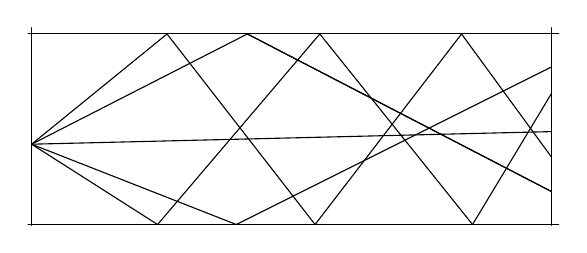
\begin{tikzpicture}[line cap=round,line join=round,>=triangle 45,x=1.0cm,y=1.0cm]
\clip(1.35,-0.01) rectangle (8.1,2.5);
\draw [domain=1.35:8.1] plot(\x,{(--2.81-0*\x)/1.16});
\draw [domain=1.35:8.1] plot(\x,{(-0-0*\x)/2.74});
\draw (1.4,-0.01) -- (1.4,2.5);
\draw (8,-0.01) -- (8,2.5);
\draw (1.4,1.02)-- (3.12,2.42);
\draw (3.12,2.42)-- (5,0);
\draw (5,0)-- (6.86,2.42);
\draw (6.86,2.42)-- (8,0.86);
\draw (1.4,1.02)-- (3,0);
\draw (3,0)-- (5.06,2.42);
\draw (5.06,2.42)-- (7,0);
\draw (7,0)-- (8,1.66);
\draw (1.4,1.02)-- (8,1.18);
\draw (1.4,1.02)-- (4,0);
\draw (4,0)-- (8,2);
\draw (1.4,1.02)-- (4.14,2.42);
\draw (4.14,2.42)-- (8,0.42);
\draw (8,0.42)-- (8,2);
\draw (4.14,2.42)-- (8,0.42);
\end{tikzpicture}
\caption{Exemples de trajet avec le multimode à saut d'indice}
\end{center}
\end{figure}

\begin{figure}[H]
\begin{center}
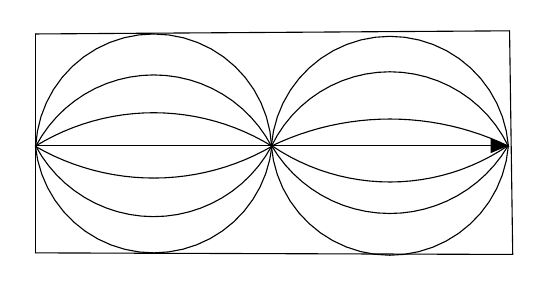
\begin{tikzpicture}[line cap=round,line join=round,>=triangle 45,x=1.0cm,y=1.0cm]
\clip(-0.1,-1.4) rectangle (6.1,1.5);
\draw [->] (0,0) -- (6,0);
\draw [shift={(1.5,-0.79)}] plot[domain=0.48:2.66,variable=\t]({1*1.69*cos(\t r)+0*1.69*sin(\t r)},{0*1.69*cos(\t r)+1*1.69*sin(\t r)});
\draw [shift={(4.5,-0.73)}] plot[domain=0.45:2.69,variable=\t]({1*1.67*cos(\t r)+0*1.67*sin(\t r)},{0*1.67*cos(\t r)+1*1.67*sin(\t r)});
\draw [shift={(1.5,0.8)}] plot[domain=3.63:5.79,variable=\t]({1*1.7*cos(\t r)+0*1.7*sin(\t r)},{0*1.7*cos(\t r)+1*1.7*sin(\t r)});
\draw [shift={(4.5,0.88)}] plot[domain=3.67:5.75,variable=\t]({1*1.74*cos(\t r)+0*1.74*sin(\t r)},{0*1.74*cos(\t r)+1*1.74*sin(\t r)});
\draw [shift={(1.5,2.59)}] plot[domain=4.19:5.24,variable=\t]({1*3*cos(\t r)+0*3*sin(\t r)},{0*3*cos(\t r)+1*3*sin(\t r)});
\draw [shift={(4.5,2.21)}] plot[domain=4.12:5.31,variable=\t]({1*2.67*cos(\t r)+0*2.67*sin(\t r)},{0*2.67*cos(\t r)+1*2.67*sin(\t r)});
\draw [shift={(1.5,-2.45)}] plot[domain=1.02:2.12,variable=\t]({1*2.87*cos(\t r)+0*2.87*sin(\t r)},{0*2.87*cos(\t r)+1*2.87*sin(\t r)});
\draw [shift={(4.5,-3.13)}] plot[domain=1.12:2.02,variable=\t]({1*3.47*cos(\t r)+0*3.47*sin(\t r)},{0*3.47*cos(\t r)+1*3.47*sin(\t r)});
\draw [shift={(1.5,0.15)}] plot[domain=3.24:6.19,variable=\t]({1*1.51*cos(\t r)+0*1.51*sin(\t r)},{0*1.51*cos(\t r)+1*1.51*sin(\t r)});
\draw [shift={(4.5,0.12)}] plot[domain=3.22:6.2,variable=\t]({1*1.51*cos(\t r)+0*1.51*sin(\t r)},{0*1.51*cos(\t r)+1*1.51*sin(\t r)});
\draw [shift={(1.5,-0.08)}] plot[domain=0.05:3.09,variable=\t]({1*1.5*cos(\t r)+0*1.5*sin(\t r)},{0*1.5*cos(\t r)+1*1.5*sin(\t r)});
\draw [shift={(4.5,-0.12)}] plot[domain=0.08:3.06,variable=\t]({1*1.51*cos(\t r)+0*1.51*sin(\t r)},{0*1.51*cos(\t r)+1*1.51*sin(\t r)});
\draw (0,1.42)-- (6.02,1.46);
\draw (0,-1.36)-- (6.06,-1.38);
\draw (6.02,1.46)-- (6.06,-1.38);
\draw (0,1.42)-- (0,-1.36);
\end{tikzpicture}
\caption{Exemples de trajet avec le multimode à gradient d'indice}
\end{center}
\end{figure}

\newpage
\section{Propagation atmosphérique et antennes}

Les ondes se propagent et interagissent avec leur environnement. Cette interaction dépend de la \textit{fréquence}, de la \textit{taille des objets} en question et de la \textit{surface} des objets. Il existe différents types de propagation:
\begin{itemize}
	\item Propagation par onde directe
	\item Propagation par onde de sol
	\item Propagation par réflexion/réfraction sur l'ionosphère
	\item Propagation par satellite
\end{itemize}
Et il existe de nombreux types d'antennes utilisé dans ces contexte.
\begin{figure}[H]
\tiny
\centering
\begin{picture}(500,162)
	%\put(0,0){\framebox(500,180)}
	% Longueur d'onde
	\put(500,152){\vector(-1,0){430}}
	\put(100,150){\line(0,1){4}} \put(90,156){1Mm}
	\put(130,150){\line(0,1){4}} \put(120,156){100km}
	\put(160,150){\line(0,1){4}} \put(153,156){10km}
	\put(190,150){\line(0,1){4}} \put(184,156){1km}
	\put(220,150){\line(0,1){4}} \put(212,156){100m}
	\put(250,150){\line(0,1){4}} \put(243,156){10m}
	\put(280,150){\line(0,1){4}} \put(275,156){1m}
	\put(310,150){\line(0,1){4}} \put(302,156){10cm}
	\put(340,150){\line(0,1){4}} \put(334,156){1cm}
	\put(370,150){\line(0,1){4}} \put(362,156){1mm}
	\put(400,150){\line(0,1){4}} \put(391,156){100$\mu$m}
	\put(430,150){\line(0,1){4}} \put(423,156){10$\mu$m}
	\put(460,150){\line(0,1){4}} \put(453,156){1$\mu$m}
	\put(0,150){Longueur d'onde}
	\put(60,150){$\lambda$}
	% Fréquence
	\put(0,130){Fréquence}
	\put(70,132){\vector(1,0){430}}
	\put(85,130){\line(0,1){4}} \put(77,122){100Hz}
	\put(115,130){\line(0,1){4}} \put(107,122){1kHz}
	\put(145,130){\line(0,1){4}} \put(134,122){10kHz}
	\put(175,130){\line(0,1){4}} \put(165,122){100kHz}
	\put(205,130){\line(0,1){4}} \put(195,122){1MHz}
	\put(235,130){\line(0,1){4}} \put(222,122){10MHz}
	\put(265,130){\line(0,1){4}} \put(251,122){100MHz}
	\put(295,130){\line(0,1){4}} \put(286,122){1GHz}
	\put(325,130){\line(0,1){4}} \put(314,122){10GHz}
	\put(355,130){\line(0,1){4}} \put(342,122){100GHz}
	\put(385,130){\line(0,1){4}} \put(376,122){1THz}
	\put(415,130){\line(0,1){4}} \put(404,122){10THz}
	\put(445,130){\line(0,1){4}} \put(432,122){100THz}
	\put(475,130){\line(0,1){4}} \put(466,122){1PHz}
	% Pointille
	\multiput(85,120)(0,-4){30}{\line(0,-1){2}}
	\multiput(115,120)(0,-4){30}{\line(0,-1){2}}
	\multiput(145,120)(0,-4){5}{\line(0,-1){2}}
	\multiput(175,120)(0,-4){5}{\line(0,-1){2}}
	\multiput(205,120)(0,-4){5}{\line(0,-1){2}}
	\multiput(235,120)(0,-4){5}{\line(0,-1){2}}
	\multiput(265,120)(0,-4){5}{\line(0,-1){2}}
	\multiput(295,120)(0,-4){5}{\line(0,-1){2}}
	\multiput(325,120)(0,-4){5}{\line(0,-1){2}}
	\multiput(355,120)(0,-4){5}{\line(0,-1){2}}
	\multiput(385,120)(0,-4){22}{\line(0,-1){2}}
	\multiput(385,16)(0,-4){4}{\line(0,-1){2}}
	\multiput(415,120)(0,-4){30}{\line(0,-1){2}}
	\multiput(445,120)(0,-4){30}{\line(0,-1){2}}
	\multiput(475,120)(0,-4){30}{\line(0,-1){2}}
	\put(130,82){\framebox(30,18){VLF}}
	\put(160,82){\framebox(30,18){LF}}\put(170,74){km}
	\put(190,82){\framebox(30,18){MF}}\put(200,74){hm}
	\put(220,82){\framebox(30,18){HF}}\put(228,74){dam}
	\put(250,82){\framebox(30,18){VHF}}\put(262,74){m}
	\put(280,82){\framebox(30,18){UHF}}\put(290,74){dm}
	\put(310,82){\framebox(30,18){SHF}}\put(320,74){cm}
	\put(340,82){\framebox(30,18){EHF}}\put(350,74){mm}
	\put(0,92){Désignation}
	\put(0,84){internationale}
	% Pointille sous boite
	\multiput(145,80)(0,-4){20}{\line(0,-1){2}}
	\multiput(175,72)(0,-4){18}{\line(0,-1){2}}
	\multiput(205,72)(0,-4){18}{\line(0,-1){2}}
	\multiput(235,72)(0,-4){18}{\line(0,-1){2}}
	\multiput(265,72)(0,-4){2}{\line(0,-1){2}}
	\multiput(265,56)(0,-4){14}{\line(0,-1){2}}
	\multiput(295,72)(0,-4){5}{\line(0,-1){2}}
	\multiput(295,44)(0,-4){11}{\line(0,-1){2}}
	\multiput(325,72)(0,-4){5}{\line(0,-1){2}}
	\multiput(325,36)(0,-4){9}{\line(0,-1){2}}
	\multiput(355,72)(0,-4){7}{\line(0,-1){2}}
	\multiput(355,24)(0,-4){6}{\line(0,-1){2}}
	% Line
  \textcolor{red}{\put(145,60){\line(1,0){90}}} \put(240,58){onde de sol}
  \textcolor{blue}{\put(175,50){\line(1,0){90}} }\put(270,48){réflection ionosphérique}
  \textcolor{orange}{\put(235,40){\line(1,0){60}}} \put(300,38){réfraction troposphérique}
  \textcolor{purple}{\put(265,30){\line(1,0){60}} }\put(330,28){dispersion troposphérique}
  \textcolor{green}{\put(235,20){\line(1,0){120}}} \put(360,18){visibilité directe}
\end{picture}
\normalsize
\caption{Les différentes techniques de propagation}
\end{figure}

\subsection{Onde directe}

Les ondes directes sont envoyés en \textbf{ligne droite} d'une antenne à
une autre. Elles ont une portée relativement limitée et il y a des
interférences avec l'onde réfléchie sur la terre. (\textit{En effet
entre deux antennes il existe deux chemins : l'un direct et l'autre avec
une réflexion de l'onde sur la terre}).

\subsection{Onde de sol}

Les ondes de sol utilisent des ondes basse fréquence qui ont tendance à
se propager le long du sol,\textit{ selon une propriété de celle ci}. En
effet, les fronts d'ondes des ondes basses fréquences se déplacent perpendiculairement au sol.
\begin{figure}[H]
\centering
\begin{tabular}{ll}
\hline
Frequence & Portée (km)\\
\hline
$100 kHz$ & $200$\\
$1 MHz$ & $60$\\
$10 MHz$ & $6$\\
$100 MHz$ & $1.5$\\
\hline
\end{tabular}
\end{figure}

\subsection{Propagation ionosphérique}

Sous l'effet de l'\textbf{ionisation} de l'air par les UV solaires, la
densité en électrons des couches de l'ionosphère les plus éloignées
augmentent. Ainsi ce \og{}mur\fg{} d'électrons cause la réfraction,
voire même la réflexion des signaux. On reconnait \textbf{4 couches
précises} (càd 4 endroits où la densité augmente de facon
particulièrement rapide). De la plus proche à la plus éloignée de la
Terre, la couche $D$, $E$, $F_1$ et $F_2$ (ces deux dernières devenant une seule pendant la nuit, la couche $F$).

Grâce à cette propagation, on peut faire \og{}rebondir\fg{} des ondes
sur ces couches et propager une onde entre les continents (au-delà de
l'horizon)\cite{Ion}. On utilise massivement cette technique pour les ondes de hautes fréquence.

\begin{description}
  \item[MUF] est la Maximal Usable Frequency, càd la fréquence maximun
      telle que l'on est sûr
    à 50\% qu'elle est réfléchie sur la ionosphère.
    Celle-ci dépend de l'activité solaire, elle est donc différente le jour et la nuit.
    (\textit{26MHz à 14h, et 20MHz à 5h})
\end{description}

\subsection{Propagation par satellite}

Pour transmettre ces signaux, on envoie des ondes directement d'une antenne à un satellite géostationnaire se trouvant sur une orbite équatoriale à $36.000km$ d'altitude. Ensuite le satellite renvoi le signal vers une antenne au sol.

\subsection{Antennes}

Une antenne est un dispositif permettant de rayonner (émetteur) ou, de
capter (récepteur), les ondes électromagnétiques\cite{WikiAntenne}. Nous
trouvons autour d'une antenne une série de champs magnétiques et de
champs électriques.

\begin{description}
\item[L' onde TEM] (appelé mode Transverse Electrique-Magnétique) est un mode de propagation tel que les champs électrique et magnétique sont tous deux orthogonaux à la direction de propagation\cite{WikiTEM}.
\item[L'antenne isotrope] est une antenne dont le diagramme de rayonnement est un cercle.
\end{description}

L'antenne envoie un rayonnement dans une certaine direction, mais
provoque aussi un rayonnement inverse non désiré. Ce rayonnement à un angle d'ouverture $\theta$. On peut mesurer le gain de l'antenne de la manière suivante:
$$Gain = \frac{puissance\ dans\ direction\ de\ puissance\ maximum}{puissance\ dans\ cette\ direction\ si\ l'antenne\ etait\ isotrope}$$

\begin{description}
  \item[L'angle d'ouverture] d'une antenne est l'angle de direction pour lequel la
    puissance rayonnée est la moitié de la puissance rayonnée dans la direction la plus
    favorable.
\end{description}

\begin{center}
\definecolor{qqwuqq}{rgb}{0,0.39,0}
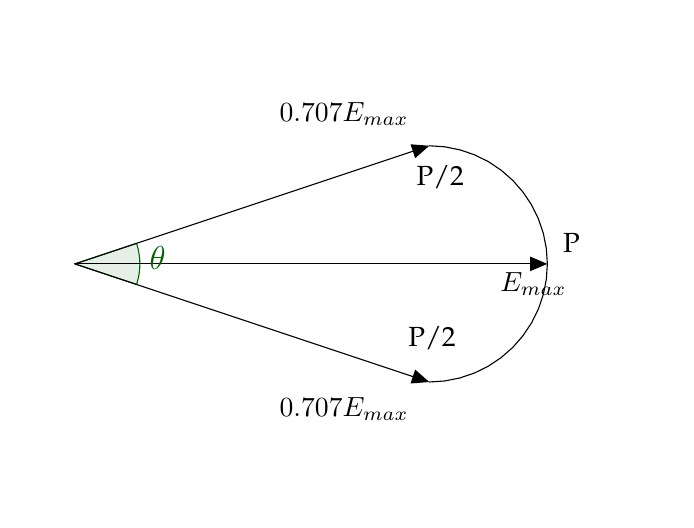
\begin{tikzpicture}[scale=1.5, line cap=round,line join=round,>=triangle 45,x=1.0cm,y=1.0cm]
\clip(-0.4,-2) rectangle (5,2);
\draw [shift={(0,0)},color=qqwuqq,fill=qqwuqq,fill opacity=0.1] (0,0) -- (-18.43:0.55) arc (-18.43:18.43:0.55) -- cycle;
\draw [->] (0,0) -- (4,0);
\draw [->] (0,0) -- (3,-1);
\draw [->] (0,0) -- (3,1);
\draw [shift={(3,0)}] plot[domain=-1.57:1.57,variable=\t]({1*1*cos(\t r)+0*1*sin(\t r)},{0*1*cos(\t r)+1*1*sin(\t r)});
\draw (3.52,0.01) node[anchor=north west] {$E_{max}$};
\draw (2.74,-0.45) node[anchor=north west] {P/2};
\draw (2.81,0.92) node[anchor=north west] {P/2};
\draw (1.65,1.45) node[anchor=north west] {$0.707E_{max}$};
\draw (1.65,-1.05) node[anchor=north west] {$0.707E_{max}$};
\draw (4.05,0.34) node[anchor=north west] {P};
\begin{scriptsize}
\draw[color=qqwuqq] (0.7,0.05) node {\large $\theta$};
\end{scriptsize}
\end{tikzpicture}
\end{center}

Voici différents types d'antenne:
\begin{itemize}
\item Dipole $\lambda/2$
\item Antenne endfire
\item Antenne yagi
\item Antenne \og{}endfire\fg{}
\item Antenne parabolique
\end{itemize}

\subsubsection{Trajets multiples}

Les antennes envoient des ondes, il arrive que ces ondes croisent des
objets (comme dit précédemment, des couches de l'atmosphère p.ex.), ces
objets reflètent les ondes et entraînent le problème des \textbf{trajets
multiples}. Les trajets multiples sont un problème courant qui fait que
le même signal arrive à des moments différents chez le récepteur,
provoquant les mêmes effets que le \textit{principe de dispersion} ainsi
qu'une désynchronisation du signal. \newline

Un signal qui varie vite a une plus grande sensibilité aux trajets
multiples.

\subsubsection{Dipole $\lambda/2$}

Un dipole est composé de deux tiges dont la taille est $\frac{\lambda}{4}$.
Les tensions sont minimales au centres et maximales sur les extrémitées.

\begin{figure}[H]
 \begin{center}
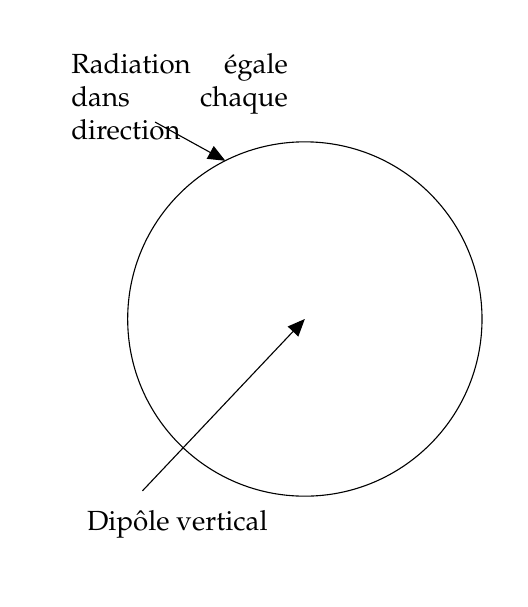
\begin{tikzpicture}[line cap=round,line join=round,>=triangle 45,x=1.0cm,y=1.0cm]
\clip(0,0) rectangle (6,7);
\draw(3.52,3.3) circle (2.25cm);
\draw [line width=3.2pt] (12.18,0.7)-- (12.18,6.68);
\draw [->] (1.46,1.12) -- (3.52,3.3);
\draw (0.63,1) node[anchor=north west] {Dipôle vertical};
\draw [->] (1.62,5.8) -- (2.51,5.31);
\draw (0.43,6.8) node[anchor=north west] {\parbox{2.75 cm}{Radiation égale dans chaque direction}};
\end{tikzpicture}
\caption{Rayonnement d'un dipôle (vue du haut)}
 \end{center}
\end{figure}

\begin{figure}[H]
\begin{center}
\definecolor{qqwuqq}{rgb}{0,0.39,0}
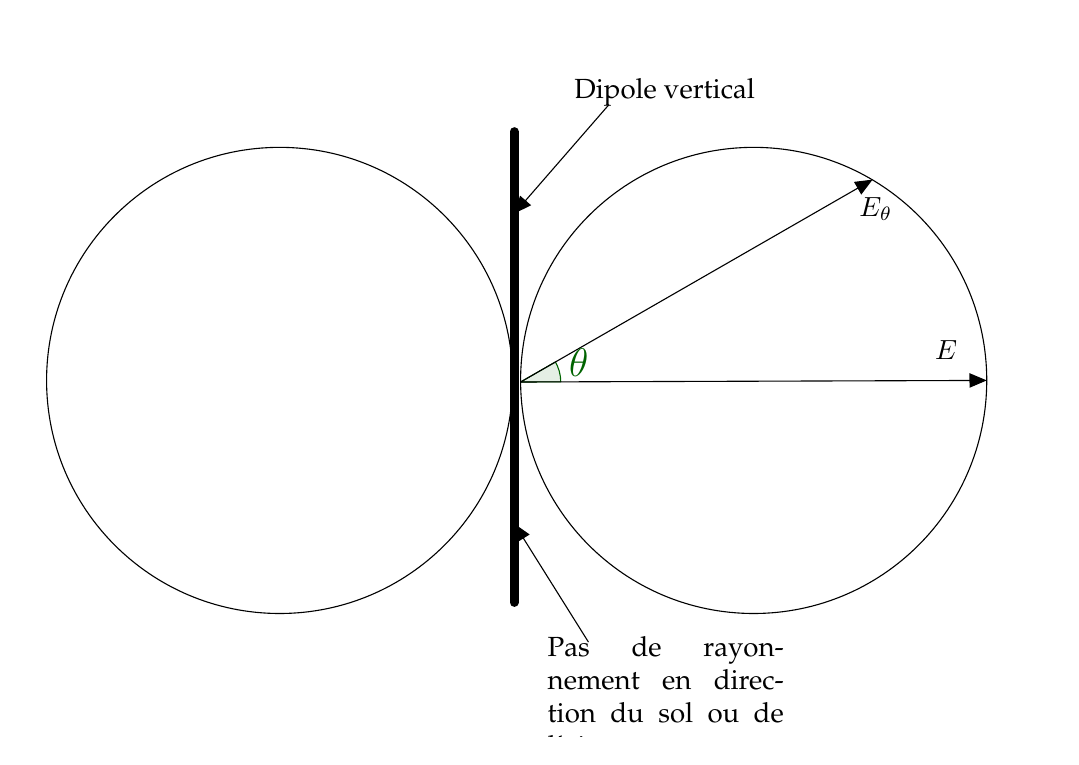
\begin{tikzpicture}[line cap=round,line join=round,>=triangle 45,x=1.0cm,y=1.0cm]
\clip(6,-1) rectangle (19,8);
\draw [shift={(12.26,3.5)},color=qqwuqq,fill=qqwuqq,fill opacity=0.1] (0,0) -- (0.19:0.51) arc (0.19:29.91:0.51) -- cycle;
\draw(3.52,3.3) circle (2.25cm);
\draw(9.2,3.52) circle (2.96cm);
\draw(15.22,3.52) circle (2.96cm);
\draw [line width=3.2pt] (12.18,0.7)-- (12.18,6.68);
\draw (0.63,1) node[anchor=north west] {Dipôle vertical};
\draw [->] (12.26,3.5) -- (18.18,3.52);
\draw [->] (12.26,3.5) -- (16.73,6.07);
\draw (16.44,5.97) node[anchor=north west] {$E_{\theta}$};
\draw (17.4,4.15) node[anchor=north west] {$E$};
\draw [->] (13.38,7.02) -- (12.18,5.64);
\draw (12.82,7.48) node[anchor=north west] {Dipole vertical};
\draw [->] (13.12,0.2) -- (12.18,1.7);
\draw (12.48,0.4) node[anchor=north west] {\parbox{3.0 cm}{Pas de rayonnement en direction du sol  ou de l'air}};
\begin{scriptsize}
\draw[color=qqwuqq] (13.0,3.74) node {\Large $\theta$};
\end{scriptsize}
\end{tikzpicture}
\caption{Rayonnement d'un dipôle (vue de côté)}
 \end{center}
\end{figure}



\subsubsection{Dipole replié}

\paragraph{Le principe du miroir} permet de n'utiliser que la moitié du fil pour
transmettre, tout simplement qu'il y a un miroir qui corresponnd à l'autre moité du fil.

L'antenne à une taille égale à $\frac{\lambda}{2}$ et permet d'avoir une bande passante
plus large.

\subsubsection{Antenne ``endfire''}

L'antenne est composé de deux ``dipole'' de longeur $\frac{\lambda}{2}$ séparé par
$\frac{\lambda}{4}$.  L'antenne de droite est alimenté avec une avance de phase de 90°
(càd $\frac{\lambda}{4}$ par rapport à celle de droite. \textbf{Cela entraine un
renforcement vers la gauche}.

\begin{center}
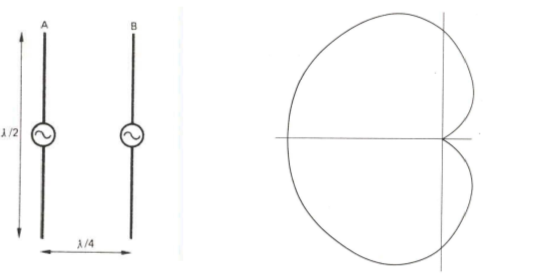
\includegraphics[width=8cm]{img/endfire.png}
\end{center}

\subsubsection{Antenne yagi (ou toit de maison)}

Une antenne Yagi est composé d'un \textbf{reflecteur}, dun \textbf{dipole} et d'un \textbf{directeur}.
La directivité d'une antenne yagi est très étroite, càd que cette antenne est précise.
Notons que cette précision diminue les parasites à la réception!

Pour augmenter la directivité d'une antenne, il faut augmenter le nombre de directeur mais
cela va diminuer la bande passante.

\begin{center}
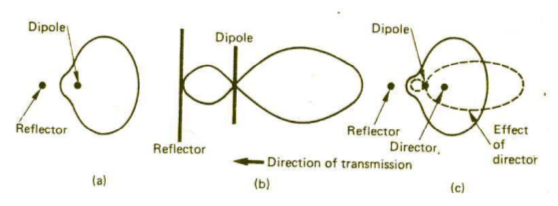
\includegraphics[width=10cm]{img/yagi.png}
\end{center}

\subsubsection{Antenne parabolique}

L'antenne parabolique utilise le principe de la parabole pour émettre/récupérer
un signal en le point central de la parabol.

\begin{center}
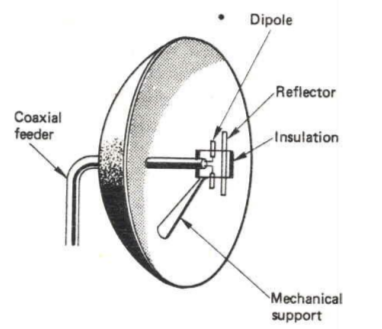
\includegraphics[width=5cm]{img/par.png}
\end{center}

\subsubsection{Réseau d'antennes}

Le réseau d'antenne est utilisé pour récupérer un signal faible (notament pour
l'aéro-spatiale) en ``agrégant'' des signaux similaires.
Attention, les antennes doivent être séparé d'un multiple de la longueur d'onde.

\begin{center}
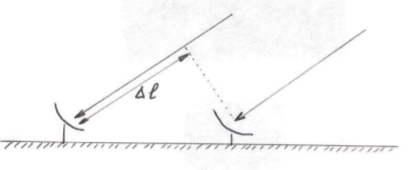
\includegraphics[width=5cm]{img/reseau.png}
\end{center}

\newpage
\section{Modulation}

La modulation va permettre de \textbf{greffer de l'information sur un signal}.
Il y a la modulation analogique et numérique.

\begin{description}
\item[La modulation] permet de transposer le signal contenant l'information
  ( appelé signal \textbf{modulant})  autour d'une autre fréquence appelé la \textbf{porteuse}.
  Le signal \textbf{modulé} ressemble à une sinusoide et la variation contient l'information du signal \textbf{modulant}.
\end{description}

Un signal est de la forme:
$$v_x(t) = A_c cos(\omega_c t + \varphi_c)$$
Il existe donc trois types de modulation, \textbf{modulation d'amplitude} (on joue sur $A_c$), \textbf{modulation de fréquence} (on joue sur $\omega$) et \textbf{modulation de phase} (on joue sur $\varphi_c$).

\subsection{Modulation en bande de base}

La transmission est dite en bande de base si elle ne subit \textbf{aucune transposition de fréquence par modulation}. Les fréquences initiales du signal émis sont donc préservées\cite{deptinfo}.


\subsection{Modulation d'amplitude (AM)}

A partir d'une \textbf{porteuse} et d'un signal \textbf{modulant} on va creer le signal \textbf{modulé} en appliquant les changements d'amplitude du signal modulant. Avec $s(t)$ le signal et l'on sait $\varphi_c = 0$, on a:
\begin{eqnarray*}
v_x(t) &=& A_c cos(\omega_c t)\\
v_{AM}(t) &=& A_c cos(\omega_c t) + ms(t)A_c cos(\omega_c t)\\
&=& A_c [1 + ms(t)] cos(\omega_c t)
\end{eqnarray*}

L'amplitude est donc multiplié par $(1+ms(t))$. Il faut faire attention de ne pas fixer $m$ (l'indice de modulation) trop grand, sinon l'on cause ce que l'on appelle de la \textbf{surmodulation}. Lors de la surmodulation la phase du signal s'inverse et il y a donc de l'ambiguité lors de la récupération du signal modulant).

\subsubsection{Démodulateur d'amplitude}

Il y a deux types de démodulateur:

\paragraph{Le detecteur d'envellope} est un circuit dont la tension descend lentement mais
augmente rapidement. Ce démodulateur nécessite un choix approprié de la constante
de temps pour la ``chute'' de la tension.

\paragraph{Le détecteur cohérent} est plus complexe est nécessite l'envoi de la fréquence
  de la porteuse.
  Ce detecteur est utilise une technique plus complexe expliqué ci dessous.

\subsubsection{Technique de modulation autour d'une porteuse utilisé pour le détecteur cohérent}
Voici un petit rappel sur les transformée de Fourier qui sera utile dans la compréhension de la suite:
\begin{eqnarray*}
f(t) &\Leftrightarrow& F(\omega)\\
f(t-t_0) &\Leftrightarrow& F(\omega)exp(-j\omega t)\\
f(t) exp(j\omega t) &\Leftrightarrow& F(\omega-\omega_0)\\
f(t) exp(-j\omega t)&\Leftrightarrow& F(\omega+\omega_0)\\
f(t) cos(\omega_0 t) &\Leftrightarrow& \frac{F(\omega-\omega_0) +F(\omega-\omega_0)}{2}
\end{eqnarray*}

\begin{figure}[H]
\centering
\begin{picture}(400,195)
%\put(0,0){\framebox(400,190)}
\put(10,15){\vector(1,0){380}}
\put(10,15){\vector(0,1){50}}
\put(393,10){$f$}
\put(20,50){Signal modulé}
\put(250,15){\vector(0,1){30}}
\put(250,11){\vector(1,0){30}}
\put(250,11){\vector(-1,0){30}}
\put(236,0){$30.000$}
\put(232,50){$600.000$}
\put(220,15){\qbezier(0,0)(15,40)(30,0)}
\put(250,15){\qbezier(0,0)(15,40)(30,0)}
\put(10,75){\vector(1,0){380}}
\put(10,75){\vector(0,1){50}}
\put(20,110){Porteuse}
\put(250,75){\vector(0,1){30}}
\put(232,110){$600.000$}
\put(393,70){$f$}
\put(10,135){\vector(1,0){380}}
\put(10,135){\vector(0,1){50}}
\put(20,170){Signal modulant}
\put(393,130){$f$}
\put(10,135){\qbezier(0,0)(15,40)(30,0)}
\end{picture}
\caption{Modulation autour d'une porteuse}
\end{figure}

Ainsi lorsque nous allons multiplier le signal par la porteuse $cos(\omega_0 t)$, si nous analysons cela en termes de transformée de Fourier, il s'agit de decaler le spectre des fréquences de $\omega_0$ dans les deux sens autour de la porteuse (en quelques sorte il y aura des fréquences "négative").

\begin{figure}[H]
  \centering
  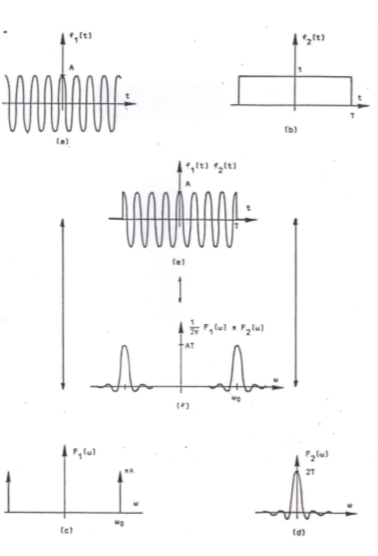
\includegraphics[width=8cm]{img/demo.png}
  \caption {Principe de démodulation selon Fourier}
\end{figure}

La fréquence de l'oscillateur local du démodulateur doit être la même
que celle du modulateur. Il y a donc intérêt d'envoyer la porteuse ou un signal qui permet de la retrouver.

\begin{figure}[H]
\centering
\begin{picture}(490,130)
\put(50,120){\textbf{Modulateur}}
\put(0,90){\vector(1,0){30}}
\put(30,70){\framebox(100,40){Product modulator}}
\put(80,40){\vector(0,1){30}}
\put(130,90){\vector(1,0){30}}
% Demodulateur
\put(300,120){\textbf{Démodulateur}}
\put(200,90){\vector(1,0){30}}
\put(230,70){\framebox(100,40){Product modulator}}
\put(230,0){\framebox(100,40){Local oscillator}}
\put(280,40){\vector(0,1){30}}
\put(330,90){\vector(1,0){30}}
\put(360,70){\framebox(100,40){Lowpass filter}}
\put(460,90){\vector(1,0){30}}
% Texte
\put(45,28){$c(t)=A_c cos(\omega_c t)$}
\put(3,78){$m(t)$}
\put(136,78){$s(t)$}
\put(206,78){$s(t)$}
\put(336,78){$v(t)$}
\put(285,52){$cos(\omega_c t + \phi)$}
\put(465,78){$v_0(t)$}
\end{picture}
\caption{Modulateur et démodulateur}
\end{figure}

Le signal sortant du démodulateur cohérent ressemble a ceci:
\begin{eqnarray*}
p(t) &=& A_c s(t) cos(\omega_c t +\varphi_c) . cos(\omega_c t + \varphi_c)\\
&=& A_c s(t) cos^2(\omega_c t + \varphi_c) \\
&=& A_c s(t) \frac{A+cos(2\omega_c t + 2\varphi_c}{2}
\end{eqnarray*}
On va filtrer en passe-bas dans le démodulateur pour récupérer $s(t)$.

\subsubsection{Bandes latérales}

Comme nous avons vu au dessus, il y a des fréquences "négatives" qui
sont envoyées, ainsi il n'est pas nécessaire d'envoyer deux fois
l'informations, l'envoi de deux bandes latérales suffit (on reconstruit
la 2e bande à la démodulation. Il y a donc pour ça deux moyens d'envoi
pour savoir quelles bandes envoyer:
\begin{itemize}
  \item USB: Upper side band (\textit{Envoi les deux aux extrémités})
  \item LSB: Lower side band (\textit{Envoi les deux aux centres})
\end{itemize}

\subsubsection{Bande latérale unique (QAM)}
On utilise l'envoi en double bande latérale dans les cas généraux mais il existe une autre technique, l'envoi en bande latéral unique par modulation en quadrature (QAM). Pour cette modulation en quadrature il faut convertir le signal $m(t)$ en deux signaux $s_1(t)$ et $s_2(t)$. Cette technique à l'avantage de diviser la bande passante nécessaire par deux (c'est utilisé pour la transmission de signaux télévisé).
$$v_{QAM}(t) = s_1(t) cos(\omega_c t) + s_2(t) sin(\omega_c t)$$
Une démodulation avec $cos(\omega_c t)$ fournit $s_1(t)$ et une démodulation avec $sin(\omega_c t)$ fournit $s_2(t)$. Evidemment le cosinus et sinus au démodulateur doit être le même qu'au modulateur.

\subsubsection{Bande latérale résiduelle}

Lorsque la bande de base s'étend jusqu'à la fréquence nulle, il n'est pas toujours possible de faire une modulation à bande latérale unique, au sens strict du terme. On peut toutefois obtenir une réduction sensible de la largeur de bande en éliminant partiellement une des deux bandes latérales. C'est la modulation à bande latérale résiduelle\cite{ulg}.

\newpage
\subsection{Modulation de fréquence(FM)}

Pour la modulation de fréquence, nous allons faire \textbf{varier la fréquence du signal modulé} en fonction du signal modulant.

D'abord la fréquence du signal envoyé est égal à la fréquence de la porteuse $\omega_c$ additionné à $k$ fois le signal modulant.
$$\omega (t) = \omega_c + ks(t)$$
Nous allons poser dans un signal $cos(\omega t + \varphi)$, la \textbf{fréquence instantané} $\beta$, tel que:
$$\beta (t) = \omega t + \varphi$$
Bien evidemment apres modulation la fréquence instantané vaut:
$$\beta (t) = \omega_c t + k s(t)( + \varphi_c$$
On a aussi la relation:
$$\omega (t) = \frac{d\beta (t)}{dt}$$

\subsubsection{Indice de modulation}

On doit définir aussi l'indice de modulation qui est égal à l'excursion maximum de fréquence du signal modulé $f_d$ (\textit{càd la variation de fréquence instantané maximale}) sur la fréquence maximun du signal modulant $f_m$ .
$$m = \frac{f_d}{f_m}$$
Cet indice de modulation va nous donner la valeur maximale de la
déviation de fréquence\cite{rennes}. La largeur de la bande passante
utilisée par le signal va varier en fonction de cet indice.\\

Exemple: \textit{la fréquence maximale d'un signal hi-fi modulant est de $15 kHz$ et les radios utilisent deux types de bandes, les Wide Band FM qui ont une excursion maximale de $75 kHz$ et donc un indice de modulation de $m=5$, et les Narrow Band FM qui ont une excursion maximale de $15 kHz$ et donc un indice de modulation $m=1$}.

Une règle empirique, la \textbf{formule de Carson} va nous permettre d'évaluer la largeur d'une bande passante d'un signal modulé en fréquence.
$$B = 2(f_d + f_m)$$

\subsubsection{Bruit}

En modulation AM nous avons un bruit constant quel que soit la
fréquence, tandis qu'en FM le bruit augmente proportionnelement avec la
fréquence. Il est toujours possible d'augmenter la qualité en augmentant
l'indice de modulation\cite{tafro} (ce qui a pour conséquence évidemment
d'augmenter le spectre du signal envoyé et donc d'encombrer la bande
passante). \newline

Mais une technique utilisé en FM pour la réduction du bruit est la \textbf{préaccentutation} avec la \textbf{désaccentutation}.
\begin{description}
	\item[La préaccentuation] consiste à favoriser les fréquences aigues par rapport au fréquence basses afin de minimiser les défauts.\cite{sonelec}. Le bruit rapporté à chaque fréquence est ainsi constant.

	\item[La désaccentutation] est le procédé inverse de la
	    préaccentuation, qui consiste à redonner à un signal audio
	    préaccentué, son contenu fréquentiel d'origine.\cite{sonelec}.
\end{description}

\subsection{Modulation de phase (PM)}

La modulation de phase est l'équivalent de FM avec la dérivée de $s(t)$
à la place de $s(t)$. En effet si l'on reprend le calcul de tantôt, l'on
obtient:
\begin{eqnarray*}
\varphi (t) &=& \varphi_c + ks(t)\\
\beta( t) &=& \omega_c t + \varphi_c + ks(t)
\end{eqnarray*}
Nous appelons dans ce contexte $\beta (t)$ \textbf{la phase instantanée}. Et nous obtenons:
\begin{eqnarray*}
\omega (t) &=& \frac{d\beta (t)}{dt}\\
&=& \omega_c + k \frac{ds(t)}{dt}
\end{eqnarray*}

\subsection{Modulation numérique}

La modulation numérique reprend les principes vu au dessus, mais les
adaptent aux deux caractéristiques des signaux numériques: ils utilisent
des valeurs discrètes (0 ou 1) et c'est à chaque coup d'horloge qu'est
envoyé une valeur. L'envoi de signal numérique permet grâce à des codes correcteurs d'erreur la \textbf{régénération}.

\subsubsection{Modes d'envois}
Les différents mode d'envoi sont les suivants:
\begin{itemize}
	\item \textbf{Amplitude Shift Keying (ASK)}: On change d'amplitude suivant le bit rencontré
	\item \textbf{Frequency Shift Keying (FSK)}: On change de fréquence suivant le bit rencontré, l'indice de modulation optimal est de $0.64$ (c'est experimental, voir schéma cours).
	\item \textbf{Phase Shift Keying (PSK)}: On change de phase suivant le bit rencontré
	\item \textbf{Differential-PSK}: l'information est contenue dans le déphasage de deux signaux successif.
\end{itemize}

\subsubsection{Mapping}

Le \textbf{mapping} transforme une séquence de bits en séquence de "symboles" complexes.
Le codage (``Constellation'')  doit prendre en compte les différentes interférence, et l'impact
qu'il a sur le débit et la probabilité d'erreur.

Exemple: \textit{le code de gray modifie uniquement le bit lorsque l'on augmente une valeur numérique, lorsque le code binaire naturel représente les nombres comme des puissance de $2$}.

\subsubsection{Mise en forme}

L'idée de base pour la mise en forme du signal est de l'envoyer durant une période $T$, on obtient une mise en forme \textit{rectangulaire}.
Le soucis c'est que le contenu fréquentiel est étalé (\textbf{sidelobes}), on risque de re-recevoir la donnée. Il y a aussi un risque d'\textbf{ISI} (inter symbol interference), le symbole envoyé risque d'interferer avec le symbole en cours de reception.

\begin{description}
	\item[Side lobes] L'envoi du signal par une antenne crée un lobe principal et des sides lobes, qui sont le signal envoyé dans les autres direction que celle prévue.
\end{description}

Ce que l'on va faire pour evite l'ISI, on peut utiliser le \textbf{critère de nyquist}.
\begin{itemize}
  \item On échantillonne au recepteur tout les bits au milieu
  \item On passe le signal à 0 tout les multiple de $T$
\end{itemize}

Cela nécessite évidemment une bonne synchronisation entre l'emetteur et le recepteur.
Le critère peut être détruit par la dispersion du canal.

\subsubsection{Réception et décision}

Lors de la réception, le signal est filtré pour retrouver le \textbf{critère de Nyquist} ou
minimiser le bruit si il n'y a pas de dispersion.
Ensuite on échantillonne au milieu.

Pour les différentes valeurs possibles des symboles nous allons prendre le symbole le plus proche dans la constellation (il reste une certaine probabilité d'erreur).

\newpage
\section{Applications}

Dans cette partie nous allons regarder l'application des principes vu tant à la radio qu'à la télévision.

\subsection{Réception superhétérodyne}

En électronique, un récepteur hétérodyne est un récepteur conçu sur le principe du mélange de fréquences, ou \textbf{hétérodynage}, pour convertir le signal reçu en une fréquence intermédiaire plus basse qu'il est plus facile d'utiliser que la fréquence reçue en direct\cite{sh}.

Il faut se ramener à une fréquence plus faible pour pouvoir amplifier et démoduler plus facilement le signal reçu\cite{sh2}.

\begin{eqnarray}
    f_{IF} &=& f_{rx} - f_{local}\\
      f_{IF} &=& f_{local} - f_{rx}
    \end{eqnarray}

    Ces deux fréquences sont donc symétrique autour de $f_{local}$, et nous récupérons
    (2) qui est la fréquence plus basse du signal reçu via un filtre passe bas.

    \paragraph{Note}: $f_{local}$ qui est la fréquence de l'oscillateur local doit être
    adapté à la fréquence du signal reçu. Si la fréquence d'un signal varie, l'oscillateur
    doit s'adapter pour que $f_{IF}$ reste constant.

\subsection{Emetteur-recepteur radio}

Dans l'emission stereo radio en FM, on envoi dans l'intervalle $0-15 kHz$ la somme des signaux $G+D$. A la fréquence de $19kHz$ un \textbf{signal pilote} qui indique que l'on utilise autour de la fréquence $38 kHz$ un signal stéréo. Le signal stéréo $G-D$ est alors envoyé en LSB en modulation AM autour de la porteuse $38kHz$.


\begin{center}
  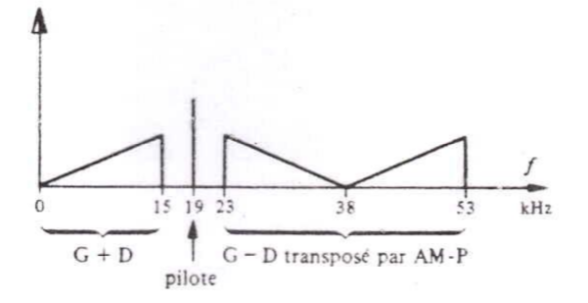
\includegraphics[width=8cm]{img/stereo.png}
\end{center}

\subsection{Emetteur-Recepteur TV noir et blanc}

\textbf{TODO}

\subsection{Télévision Couleurs}

Différents format sont utilisé pour l'envoi de la télévision analogique, il s'agit de \textbf{NTSC} (USA, Japon, Canada, ...), \textbf{PAL} (Uk, Allemagne) et \textbf{SECAM} (France, URSS, ...). Afin de conserver la compatibilité avec les télévision en noir et blanc, on sépare l'envoi de la luminance et de la chrominance (voir section 1).

Il y a deux types d'envoi de couleurs en fait, YUV et YIQ. Y la luminance est la même dans les deux cas, mais pas IQ et UV.
\begin{eqnarray*}
U &=& 0.493 (B - Y)\\
V &=& 0.877 (R - Y)\\
Q &=& 0.41(B-Y)+0.48(R-Y)\\
I &=& -0.27(B-Y)+0.74(R-Y)
\end{eqnarray*}

\subsubsection{NTSC}

En NTSC, on envoi le son en FM, la chrominance en QAM et la luminance en VSB (bande latérale résiduelle). Ce systeme utilise l'envoi des chrominance en IQ

\subsubsection{PAL (phase alternating line)}

PAL envoi les couleurs en utilisant le système YUV. La chrominance est envoyé de la maniere suivante $v(t)=U sin(\omega_c t) \pm V cos(\omega_c t)$. Le système PAL à les caractéristiques suivantes: U et V possède la même largeur de bande, la porteuse son est plus éloigné de la porteuse de l'image et le spectre est plus compliqué.

\subsubsection{Secam (séquentiel à mémoire)}

On transmets chaque chrominance qu'une ligne sur deux et on complète avec la ligne précédente. Ainsi, en SECAM, la résolution en chrominance est moitié moindre que la résolution en luminance (celle de l’image en noir-et-blanc). En pratique, cela ne pose pas de problème particulier, car l’œil humain présente à peu près les mêmes caractéristiques\cite{SECAM}. On va aussi éviter les modulations en FM.

\subsection{Télévision numérique}

En binaire, les couleurs sont envoyé sur 8 bits (256 valeurs), ainsi l'envoi des couleurs est un peu différents.
\begin{eqnarray*}
y&=&0.299 r + 0.587 g + 0.114 b\\
Y&=&219y + 16\\
CR&=&\frac{112(r-y)}{0.701}+128\\
CB&=&\frac{112(b-y)}{0.886}+128
\end{eqnarray*}
$Y$ est échantilloné à $13.5MHz$ (864 échantillonage par ligne) et les chrominances à $6.75MHz$ (la moitié). On envoi 8 bits par échantillon, des lors il nous faut une bande passante, avant compression, de $216Mbit/s$ (c'est relativement énorme).

Voici les différents avantages et désavantages de la télévision numérique:
\begin{itemize}
\item[+]Compression
\item[+]Codes correcteurs d'erreur
\item[+]Enregistrement et stockage
\item[-]Delais de zapping
\item[-]Dégradation rapide si mauvais signal
\end{itemize}

\newpage
\section{OSI}

Le modèle de couches OSI (ou Open Systems Interconnection) est un standard de communication en réseau de tout les système informatique, il utilise 7 niveaux différents. Il s'agit d'un système de communation de paquets. Chaque niveau sait lire le contenu d'un même niveau car ils utilisent un même \textbf{protocole} de communication (un même language).

Voici les différents niveaux:
\begin{enumerate}
\item Physique
\item Liaison
\item Réseau
\item Transport
\item Session
\item Présentation
\item Application
\end{enumerate}

\subsection{Niveau 1: Physique}

C'est le niveau physique, il s'agit des cables qui transporte les bits et les différents composants physiques.

\subsection{Niveau 2: Liaison}

Transporte des \textbf{trames} (bloc de données), ajoute des indications de service (flags, début, fin), s'occupe d'ajouter les codes détecteurs d'erreurs et corrige les erreurs. Ce niveau recoit les demandes de couche réseau et utilise la couche physique.

\subsubsection{Protocoles de liaison}

Le protocole définit le format de la trame, c'est à dire quels bits de controle vont où dans chaque bloc de donnée.

\begin{description}
  \item[Bit stuffing] Le bit stuffing consiste en l'insertion de bits, qui ne contiennent pas d'information. Dans le contexte du HDLC, il s'agit de limiter le nombre de bits de valeur 1 qui se suivent, car trop de 1 qui se suivent cause un signal constant et le bit stuffing va permettre la synchronisation des horloges. Un petit désavantage est que la vitesse de transmission des données va varier en fonction des données.

    On réalise le bit stuffing aussi pour pouvoir reconnaitre le début et la fin d'une trame avec les $01111110$. On empeche d'avoir d'autre séquence de 1 de cet taille dans la trame.
\end{description}


\paragraph{Exemple :}
Le protocole HDLC qui peut utiliser du bit stuffing.

\begin{figure}[H]
\centering
\begin{picture}(500,40)
\put(0,34){Bits}
\put(40,0){\framebox(60,30){01111110}}
\put(100,0){\framebox(60,30){Address}}
\put(160,0){\framebox(60,30){Control}}
\put(220,0){\framebox(80,30){Data}}
\put(300,0){\framebox(140,30){Checksum}}
\put(440,0){\framebox(60,30){01111110}}
\put(67,34){8}
\put(127,34){8}
\put(187,34){8}
\put(250,34){$\geq 0$}
\put(367,34){16}
\put(467,34){8}
\end{picture}
\caption{Protocole HDLC}
\end{figure}

Il y a 3 roles important dans le protocole de liaison de niveau 2 pour HDLC :
\begin{itemize}
\item \textbf{MAC}(Medium access control): il s'agit d'une adresse unique à chaque carte réseau qui va permetre l'acces au réseau. Ca sert d'interface entre la partie physique de l'ordinateur et les logiciels.
\item \textbf{FEC}(Forward error correction): code correcteur d'erreur
\item \textbf{ARQ}(Automatic repeat request): mécanisme de retransmission
\end{itemize}

Il y 3 types de trame spécifié par le champ de contrôle pour HDLC :
\begin{itemize}
  \item (0) (Sequ) (P/F) (Next)  : \textbf{La trame d'information} transporte les données fournies par la couche réseau (3).
  \item (1) (0) (Type) (P/F) (Next) : \textbf{La trame de supervision} transportent des commandes ou des réponses liés au contrôle d'erreurs et au contrôle de flux.
  \item (1) (1) (Type) (P/F) (Modifier) : \textbf{La trame non-numéroté} transportent des cimmandes ou réponses liés à la gestion de liaison.
\end{itemize}

\begin{description}
  \item[P/F] : ``Poll/Final'' vaut P si la trame est une commande, et F si c'est une réponse
  \item[Sequ] : numéro de la trame courante
  \item[Next] : numéro de la trame qui doit répondre
\end{description}

\subsubsection{Multiplexage}

Comme expliqué dans la section 1, le multiplexage permet le partage d'un certain canal de communication. Il existe plusieurs types de multiplexage:
\begin{itemize}
\item \textbf{TDMA}(Time division multiple access): il s'agit de diviser le temps en plusieurs périodes de temps qui seront utilisé par différents utilisateurs (time slice).
\item \textbf{FDMA}(Frequency division multiple access): une fréquence par utilisateur et plusieurs fréquence pour toute la bande.
  \item \textbf{CDMA}(Code division multiple access): Chaque utilisateur à une clé (ou code) à l'aide de laquelle son message est codé (\textit{via un XOR}) avant d'être émis. Il est important de noter que chaque utilisateur émet sur toute la largeur de la bande.
\end{itemize}

\subsection{Niveau 3: Réseau}

Transporte des paquets et traites les adressses, c'est ce niveau qui établit les trajets dans le réseau et s'occupe du trafic, des priorités et de la connexion inter réseau.

\subsection{Niveau 4: Transport}

Liens des ordinateurs via le réseau, controle les flux de données.

\subsection{Autres modèles}

Le modèle TCP/IP est aussi très utilisé, il utilise la même idée de travail en couches.

\newpage
\section{Codes correcteurs d'erreur}

L'envoi de donnée sous forme binaire permet d'avoir des codes correcteurs d'erreur. Il existe plusieurs causes pouvant causer une erreur (bruit, diaphonie, perte de synchronisation, ...).

\subsection{Code de parité}

On va compter le nombre de bit à 1 dans un groupes de n bits et rajouter à la fin de ce groupe si ce nombre est pair (0) ou impair (1). Cette technique est simple et permet la détection d'erreur, mais pas la réstoration.

\paragraph{Note :} Si une ligne contient un nombre pair d'erreurs, elles ne seront pas détectée.

\subsection{Code de parité étendu}

On peut ajouter de la parité à la fin des lignes de n bits et rajouter une ligne, ce qui transforme nos lignes en une sorte de tableau.

\paragraph{Note}: Ce code de parité étendu permet de détecter beaucoup plus d'erreur.

\subsection{Dictionnaire de mots}

On crée un dictionnaire avec différents bits qui représente des mots et si un code ne se trouve pas dans le dictionnaire, il s'agit d'une erreur. On peut alors le corriger (sauf si l'erreur crée un mots lui aussi présent dans le dictionnaire).

\subsection{Code à répétition}

Un code à simple répétition permet la détection d'erreur mais pas la correction. Un code à double répétition permet une correction et une détection simple. Plus on ajoute de redondance, plus la correction sera effective, maintenant cela à un coût élevé en terme de débit.

\subsection{Théorie des codes}

``Comment ajouter de la redondance ou définir un dictionnaire de facon à ce que ca impact le moins possible le débit.''
\textbf{Distance de Hamming}: le nombre de bits différents entre 2 mots.\\

Soient $k$ le nombre de \textbf{bits utile} et $n$ tel que $n-k$ est le nombre de \textbf{bits de controle}.
Le \textbf{taux du code} est de $k/n$. On va choisir dans le dictionnaire le mots le plus proche trouvé en utilisant la distance.

\textbf{Un code(n,k)} et de distance minimale $d$ détecte les erreurs d'ordre $d-1$ et corrige les erreurs d'ordre $floor[(d-1)/2]$.

\subsubsection{Code linéaire}

On veut trouver des codes avec une distance minimale voulue et comportant le plus de mots possible. Avec un \textbf{mot d'information}
$$i = (i_1, i_2, i_3, ..., i_k)$$
on trouve une \textbf{matrice génératrice}
$$G = (I_k; P)$$
et on calcule le \textbf{mot de code}
$$c = (i_1, i_2, ..., i_k, c_1, c_2, ..., c_{k-n}) = iG$$
Enfin on récupère la \textbf{matrice de controle}
$$H=(P^T; I_{n-k})$$
et le \textbf{syndrome}
$$s= cH^T$$
Si $s=0$ pas d'erreur détecté. Ce qui est envoyé c'est $c$. Pour trouver la matrice de parité $P$ on récupère $p_1$, $p_2$ et $p_3$ dans la matrice suivante\cite{hamming}:
\begin{figure}[H]
\centering
\begin{tabular}{c|cccc}
 & $d_1$ & $d_2$ & $d_3$ & $d_4$\\
\hline
$p_1$ & x & 1 & 1 & 1\\
$p_2$ & 1 & x & 1 & 1\\
$p_3$ & 1 & 1 & x & 1\\
$p_4$ & 1 & 1 & 1 & x\\
\end{tabular}
\end{figure}

\subsubsection{Code cyclique}

\begin{description}
  \item{Un mot binaire est un polynome $(1 0 1 1) = 1x^3 + 0x^2 + 1x + 1$.}
  \item{On a donc $i(x)$ un \textbf{polynome} de degré $k-1$. Soit $g(x)$ un \textbf{polynome générateur} de degré $n-k$.}
  \item{Si l'on divise $x^{n-k}i(x)$ par $g(x)$ le \textbf{reste} est un polynome de degré $n-k-1$. }
\end{description}

On va transmettre $c(x) = x^{n-k}i(x)-r(x)$ et vérifier qu'il est bien divisible par $g(x)$.
Si une erreur $E(x)$ intervient dans le signal transmis $T(x)$, on reçoit $R(x) = T(x) + E(x)$. Si $E(x)$ est divisible par $g(x)$ on ne verra pas qu'il y a une erreur.

\subsubsection{Code de Hamming}

On place les bits de codage aux rangs "puissances de 2". Et on fait la somme des numeros des bits à 1 (voir exemple), sans tenir compte des bits de codage.

Augmenter la taille du bloc donne généralement de meilleures performance
pour un même taux, mais la complexité de comparaison avec les
\og{}mots\fg{} existants et le délai (remplissage du 1er bloc avant
d'afficher l'image) augmentent.

Si on est dans un environnement qui provoque peu d'erreurs (\textit{bit error
rate} faible) et dans lequel la taille des blocs est faible, on préfèrera utiliser des codes détecteurs d'erreurs
plutôt que des codes correcteurs pour des raisons de performance (moins de
bit de contrôle).

\subsection{Mécanisme ARQ}

On envoie les données avec des bits de détection et il y a retour d'un message ACK qui est renvoyé si les données transmises ont été correctement reçues. Si elles ne l'ont pas été on renvoie la trame en question.

\begin{description}
  \item[ACK] : le message a bien été reçu
  \item[NACK] : le message n'a pas bien été reçu
\end{description}

\begin{description}
  \item{En mode \textbf{Stop-and-Wait} on attend le ``ACK'' de retour à chaque trame pendant un
  laps de temps. Si celui-ci est dépassé, la trame est renvoyé.}

\item{En mode \textbf{go-back-n}, on envoit les données sans attendre le ``ACK'' entre deux envois de trame. (\textit{çad que plusieurs trame sont envoyé avant de recevoir le ``ACK'' de la première})
  Si il y a un sousic de récption, on reprend l'envoi \textbf{depuis} le package qui a foiré! }

  \item{En mode \textbf{selective-repeat}, les données sont aussi envoyé sans attendre le ``ACK''
    entre deux envois de trame. Lorsque qu'elle reçoit un ``NACK'' pour une trame, elle ne
    renvoit \textbf{que} la trame en question.
  Les trames qui ont été réceptionné entre temps sont mise dans un buffer.}

\end{description}

\paragraph{Note}: Si l'ACK est long à envoyer il faut tacher d'envoyer des blocs plus long. Il faut donc bien choisir la taille des blocks et le nombre de bits de parités.

\newpage
\section{Compression}

L'audio, les images et les videos demandent énormément de place pour leur stockage, il serait impossible de stocker les données totalement décompressée (exemple: \textit{50 films de 1 minutes en 480p font 82GB}). Les proportions de compressions sont les suivantes:
\begin{itemize}
\item Texte ($2:1$)
\item Images ($5:1$)
\item Son stéréo ($6:1$)
\item Vidéo ($50:1$)
\end{itemize}

Il existe deux types de compressions: \textit{avec pertes} (lossy) et \textit{sans pertes} (lossless). Les deux principes de la compressions sont: \textbf{suppression de la redondance} et \textbf{conservation des caractéristiques importantes}.

\subsection{Codage sans pertes}

\subsubsection{Codage entropique}

Le principe du codage entropique est d'utiliser des codes courts pour des mots qui sont redondants. Il se base sur le concept d'entropie de Shannon
\begin{description}
\item[Entropie] limite théorique de l'information que l'on peut transmettre sur un canal.
\end{description}

\subsubsection{Code de Huffman}

On va former un nouvel alphabet de lettre en construisant un arbre sur base de la probabilité de voir une lettre (on observe sur le message habituellement). L'arbre est organisé tel que la branche de gauche est 0 et celle de droite 1. On commence en haut de l'arbre on mets la lettre la plus probable à gauche et le reste à droite. et on refait ca à chaque niveau.

On envoie le dictionnaire au début de la transmission.

\subsubsection{Lempel-Ziv(L77)}

C'est le codage de winzip et gzip. On regarde les données précédemment envoyé et on trouve le bout déja envoyé, on va spécifier à quel distance il se situe du points actuel et sur quel longueur il s'étend.

\subsection{Codage avec pertes}

On va mesurer une distorsion (somme carré des erreurs ou distance de hamming) qui va permettre de dire si le taux d'erreur est acceptable. Plus on admet un taux d'erreur élevé, moins on a besoin de débit pour les données.

\subsubsection{JPEG}

On remplace les blocs de 8x8 pixels par des matrices de coefficients DCT de taille 8x8. Cette compression est sans pertes, mais ca ne compresse pas! Le but en fait va être de ne prendre q'uune partie des blocs de DCT. Virer des pixels dans l'image serait impensable, oublié un bloc DCT n'est pas grave.

Dans la matrice DCT il y a une fonction cosinus représenté en deux dimensions et de facon discrete (voir la référence)\cite{dct}.

Après avoir transformé la matrice de pixel en matrice de coefficient DCT on applique la \textbf{quantification}. On divise la matrice de coéfficient par une matrice de quantification dans le but d'attenuer les hautes fréquences (fréquences auxquels l'oeil humain est très peu sensible)\cite{dct2}. Certains coefficient sont souvent ramené à 0 (ceux en bas à droite de la matrice). Apres un codage en ZIG-ZAG permet de ne garder qu'un minimum de coéfficient et de se débarasser des nuls.

\subsection{Video}

La compression vidéo utilise le principe de prédiction (via \textbf{Block Matching Algorithm}).
Ce concept se base sur l'idée que deux images successive ont habituellement très peu de différence. De temps en temps, lors d'un changement de scene, il faut evidemment conserver une image complete.

La compression vidéo se passe donc comme la JPEG mais avec une prédiction temporelle en plus, il y a 3 types de frames:
\begin{enumerate}
\item Intraframe: image complète
\item Interframe: image prédite à partir d'une précédente
\item Bidirect: image prédite à partir d'une précédente ou d'une suivante
\end{enumerate}
La prédiction consiste en fait dans la translation d'une série de bloc appartenant à l'image précédente utilisée.

\newpage
\section{GSM}

Le système GSM se base sur un système de cellules hexagonnales de
tailles différentes:
\begin{itemize}
	\item Macrocell: 30km
	\item Microcell: 2-3km
	\item Picocell: 200m
	\item Femtocell
\end{itemize}

Le système est structuré en tours de transmissions associé à une
cellule, les \textbf{BTS} (base transceiver station). Ces tours sont
associées en groupes à une station, les \textbf{BCS}(base station
controller). Enfin ces controlleurs sont associés à un centre de type
\textbf{MSC} (mobile service switching center), ces centres étant reliés
à internet pour la 3G. Evidemment, l'utilisateur communique avec les BTS.

\subsection{Réutilisation des fréquences}

On va fixer un niveau admissible d'interférence entre les différentes tours de communication (vu qu'elles utilisent les mêmes fréquences). Habituellement on limite ce taux à $\sim10 db$. On va donc placer les cellules pour que ce taux ne soit pas trop élevé.

Le \textbf{planning des fréquences} va essayer de distribuer les fréquences entre les tours de facon à éviter que des cellules voisines aient des fréquences communes.

Les bandes fréquences GSM \textbf{montantes} vont de \textcolor{red}{890 à 915 $MHz$} et \textbf{déscendantes} de \textcolor{red}{935 à 960 $MHz$}.

\subsection{Modulation}

Le système GSM utilise le \textbf{GMSK} (Gaussian minimun shift keying) pour l'envoi des données numériques. Ce système de type FSK diminue la taille de la phase de -90 degré si un 0 est rencontré et +90 degré si un 1 est rencontré. Robuste mais pas très efficace!


La largeur de la bande est de 200kHz.

\subsection{Multiplexage}

Le multiplexage GSM est un couplage du TDMA et du FDMA. Chaque tour fournit 8 timeslots et 124 canaux de 200 kHz de large. Le débit de la voix est d'environ $13kb/s$ et des données $9 kb/s$.
(Avec les code correcteurs d'erreurs).

Deux utilisateurs peuvent partager un timeslot (\textbf{half rate}, c'est à dire chacun son tour). Il y a un petit décalage entre les timeslots déscendant et montant.

\subsubsection{Structure timeslot}

Il existe 5 types de paquets (\textbf{burst}), l'emission d'un paquets correspond à l'émission de \textcolor{red}{156.25 bits}:
\begin{enumerate}
  \item \textbf{Acces}: demande de contact avec le réseau
  \item \textbf{Synchronisation}: localisation + réception d'une fréquence pour communiquer
  \item \textbf{Normal}: Envoi du message
  \item \textbf{Correction fréquence}: prévention d'interférence possible (il s'agit d'un burst vide)
  \item \textbf{Bourrage}: complete le vide
\end{enumerate}

\subsection{Dispersion}

Le problème de \textbf{dispersion} est le problème de la perte du signal entre la tours et l'utilisateur. Les causes sont multiples:
\begin{itemize}
  \item \textbf{Multi-trajets}: le signal prends plusieurs chemin pour rejoindre la station et cause des interférences. (\textit{Par exemple : rebond sur un immeuble et chemin direct})
  \item \textbf{Shadowing}: un objet obstrue la transmission
  \item \textbf{Effet Doppler}: Décalage de fréquence d'une onde entre
      l'émission et la réception quand la distance entre les deux varie
      au cours du temps. Cet effet est causé par le déplacement de
      l'utilisateur par rapport à l'antenne (c'est l'effet qu'on a quand
      on entend une sirène dans la rue, mesurer cet effet permet de
      déterminer la vitesse)
\end{itemize}

Différentes solutions sont possible. Les \textbf{codes correcteurs d'erreur} ou encore diversifier les fréquences du signal grace au \textbf{frequency hopping}. Jouer sur la \textbf{modulation} ou sur l'\textbf{égalisation} du signal.

\begin{description}
\item[Frequency hopping] On transmets le premier burst à une fréquence $f_1$, le deuxieme à une fréquence $f_2$ et le troisième à une fréquence $f_3$ et on réutilise dans cet ordre les différentes fréquences.
\end{description}

\subsection{Alignement dynamique}

Si deux utilisateurs utilisent des timeslots différentes mais que leur distance à la tour varie, il n'est pas impossible que leurs signaux s'interfère. Il faut donc procéder à l'\textbf{alignement dynamique}.

On doit adapter le time slot en fonction du temps que le signal va prendre pour arriver à la tour. Cela revient à ajouter du décalage temporel de façon à ce que la station de base tombe toujours
bien sur le timeslot qu'il faut.

L'alignement dynamique ne se fait qu'en \textbf{montant} car il peut y avoir plusieurs utilisateurs.
En effet, en \textbf{descendant} se serait ridicule puisqu'il n'y a qu'un seul destinataire possible (à savoir le gsm)!

(\textit{En gros le gsm ne parle qu'a la station alors que la station parle à beaucoup de gsm})

\subsubsection{Puissance}

La puissance d'un mobile est d'environ $2W$ quand la puissance d'une tour est de $10-50W$. Le controle de la puissance est justifié par la consommation electrique (que l'on veut minimal pour sauver les ours polaire qui crève sur la banquise) et car l'on désire avoir un bon rapport signal/bruit avec les différents utilisateurs\cite{radioelec}. Suivant leur distance à la tour une puissance différentes est nécessaire (\textbf{On ajuste par pas de 2dB}).

\subsection{Accès au système}

La premiere connexion à la tour se passe de la manière suivante: le mobile regarde les canaux
et quand il en trouve un libre il parle à la station qui va lui attribuer un canal et un timeslot. Cette procédure arrive lors de:
\begin{itemize}
\item La première connexion
\item Pour initier un appel
\item Pour répondre à un appel
\item Envoyer ou recevoir des données
\end{itemize}

\begin{description}
  \item[Handover] : Le mobile change de BTS en brisant l'ancienne et puis crée la nouvelle liaison
  \item[Soft handover] : Le mobile garde l'ancienne liaison en créant la nouvelle liaison
\end{description}

Lors de la diminution de la qualité dans un BTS, le système propose d'autre canaux de communication et le mobile effectue un \textbf{handover} pour changer de BTS vers un signal plus fort.

\subsection{Internet sur GSM}

\subsubsection{GPRS (2.5G)}
Le système GPRS utilise les paquets de transmission pour transmettre internet et l'on ne transmet un paquet que si celui-ci est nécessaire (c'est facturé au volume).

\subsubsection{Edge (2.75G)}
On passe vers une modulation 8-PSK (une transition de phase par groupes de 3 bits) qui permet
\textbf{3 à 4 fois plus de débit}. Ce type de communication implique du matériel adapté sur les stations et les terminaux mobiles.

Vitesse:
\begin{itemize}
\item 384 kbit/s pour les stations fixes (piétons et véhicules lents)
\item 144 kbit/s pour les stations mobiles (véhicules rapides)\cite{ccm}
\end{itemize}

\subsubsection{UMTS (3G)}

Changement de bande de fréquence vers des fréquence de 1885 à 2025 MHz en débit montant et 2110 à 2200 MHz en débit déscendant. La compatibilité du système est mondial. La largeur de la bande est de 5Mhz.

On utilise un \textbf{W-CDMA} (un autre type de CDMA, W c'est pour Wideband).
\begin{itemize}
  \item {Plus d'alignement dynamique nécessaire}
  \item {Soft handover possible}
  \item {Plus d'inteférence}
\end{itemize}


Vitesse:
\begin{itemize}
\item 2 Mb/s pour les stations fixes (piétons et véhicules lents)
\item 144 kbit/s pour les stations mobiles (véhicules rapides)\cite{ccm}
\end{itemize}

\newpage
\section{Wifi}

Le wifi débute en 2000, il existe de nombreux standard différents (802.11a,b,g,n,...). WLAN (Wireless Local Area Network), il s'agit en fait d'un réseau d'une seul cellule sur lequel les utilisateurs sont séparés en fréquence (FDMA). La bande de wifi est autour de 2.4GHz avec 14 bandes de 5 Mhz avec un débit de 1 à 11Mb/s.

\textbf{IEEE 802.11a} possede une fréquence de 5GHz avec des bandes de 20MHz et un débit de 6 à 50 Mb/s (mais le matériel pour ce type de transmission est très différent).

\subsection{Modulation}

La modulation se faisait en \textbf{DSSS}, aujourd'hui les nouveaux standards remplacent DSSS par OFDM. DSSS utilise du CDMA et possede une largeur de bande de 22Mhz, cette largeur couvre plusieurs canaux.

Les nouveaux standards \textbf{OFDM} utilisent une sorte de FDMA. La bande est divisée en beaucoup de petites sous-bandes qui sont rendues indépendantes par le traitement du signal. Ce qui a un énorme impact sur la bande passante.

Le standard du futur est le \textbf{MIMO} (multiple input multiple output). Cette technique utilise plusieurs antennes en même temps. Ce standard lève 3 soucis de design:
\begin{itemize}
\item Beamforming
\item Multiplexage spatial
\item Combattre les évanouissement
\end{itemize}

\subsubsection{Beamforming}

Beamforming est la technique utilisé par ces nouveaux systeme qui utilise plusieurs antennes dans une même direction pour former un réseau d'antenne. Ce reseau va envoyer un ensemble de signaux constructeur/destructeur lorsqu'ils s'interefere pour former le signal. Tout ca est une question de timing.

\subsubsection{Multiplexage spatial}

Les messages divisé doivent être réassemblé pour récuperer le canal sur lequel transite les données.

\begin{center}
  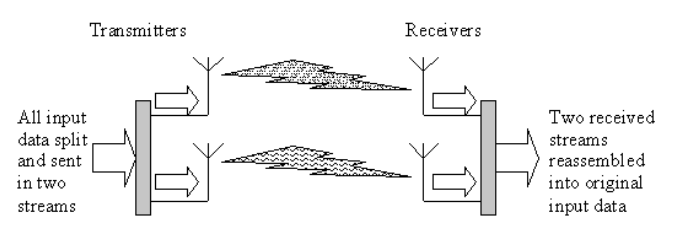
\includegraphics[width=10cm]{img/spatial.png}
\end{center}

\subsubsection{Combattre les évanouissement}

La réception peut varier énormément d'un endroit à un autre. Comme il y a plusieurs antenne envoyant un signal il y a la possiblité qu'un signal arrive et l'on choisis le meilleur signal arrivant. Il faut évidemement que les antennes soit suffisement espacé (Au moins $\frac{\lambda}{2}$).

On lutte donc contre les \textbf{trajets multiples}!

\subsection{Standards}
\begin{center}
\begin{tabular}{ccccc}
Nom & Fréquence & Modulation & Bande Passante & Portée\\
\hline
802.11a & 5.0GHz & OFDM & 30Mb/s & 10m\\
802.11b & 2.4GHz & OFDM & 6Mb/s & 100m\\
802.11g & 2.4GHz & OFDM & 30Mb/s & 100m\\
802.11n & 2.4 - 5.0GHz& MIMO & 450Mb/s & \\
\hline
\end{tabular}
\end{center}

\newpage
\section{Cryptographie}

Alors la cryptographie a deux buts: \textbf{confidentialité} et \textbf{contrer les messages frauduleux}. Il existe dans ce but différentes technique de codage. Les codes peuvent être \textbf{inconditionnelement sûrs} (théoriquement impossible à casser) ou \textbf{pratiquement sûrs} (cela prends trop de temps à casser).

\subsection{Cryptages}

On peut attaquer un code si l'on connait la clef, ou bien si l'on connais la structure du texte chiffré ou si l'on connais le texte de base et le texte chiffré.

Il existe deux types de code, les premiers sont \textbf{symétriques}, une clef permet le déchiffrement et le chiffrement et cette clef est connues des deux parties. Les seconds sont \textbf{asymétrique}, il existe une clef privé pour le déchiffrage et une clef publique pour le chiffrage.

\subsubsection{Code Jules César}

On va simplement augmenter les lettres suivant une cle. Exemple: \textit{avec une clef 3 et la lettre A, on obtiens la lettre C}.

\subsubsection{Code Vigenère}

On a une série de cle ``Jules César'' que l'on va appliquer l'une après l'autre
aux lettres à crypter.
(\textit{La premiière valeur à la première lettre, la deuxième à la deuxième, etc}).

\subsubsection{Code de Vernam}

Le \textit{xor} logique à comme propriété de pouvoir servir de clef. Un \textit{xor} avec une clef binaire et un mots renvoi un mots codé, et le \textit{xor} avec le mots codé et la clef renvois le mots de base.

Cette technique est dans une des 4 conditions suivantes:
\begin{itemize}
\item La clé est une séquence aléatoire
\item La clé est aussi longue que le message
\item La clé n'est pas réutilisé
\item La clé est disponible à l'émétteur et au recepteur (parfait pour l'armée c'est simple et éfficace).
\end{itemize}

\subsubsection{Code DES}

On dispose d'un bloc de 64 bits et d'une clef de 56 bits (et 8 bits de parité). Ca n'est plus utilisé aujourd'hui du fait qu'il peut être cassable avec la puissance de nos machine.

La technique se déroule de la manière suivante\cite{des}:
\begin{enumerate}
\item On crée une table de 8x8 bits, on démarre en haut à gauche et on mets le $58^e$ bit puis on va à droite et on mets le $50^e$ bit et on continue ainsi jusqu'au $7^e$ bit tout en bas à droite.
\item On divise la table en deux blocs de 4x8 bits, que l'on va appeller $L_0$ et $R_0$.
\item On procède à 16 opérations de permutation et de substitution basé sur des clés de 48 bits. On va transformer le groupe de droite en un groupe de 48 bits pour cela.
\item On rejoins les parties gauche et droit e et on fait l'operation inverse de la permutation du début.
\end{enumerate}

\subsubsection{Code AES}

Système plus robuste que DES mais qui utilise le même principe que DES. Cette technique admet des clés plus grande (128, 192, 256 bits).

\subsection{Algorithmes symétriques}

Les algorithme symétriques utilise souvent des opérations mathématique simple et des opérations inversible. Le soucis évident est le partage de clef sur ce type d'algorithme.


\subsection{Algorithmes asymétriques}

Ce genre d'algorithme utilise donc une clef publique et une clef privé. La clef publique permet le cryptage et la clef privé le décryptage. Ce genre d'algorithme est plus complexe et lent mais il résoud le problème du partage des clefs, tout en ajoutant le problème du fait que l'on ne sait jamais qui a envoyé le message.

La condition pour que cela fonctionne est que la clef privé soit très difficile à trouver à partir de la clef publique.

\subsubsection{Algorithmes hybride}

Pour résoudre les défauts des deux algorithme, on utilise des algorithmes \textbf{hybride} qui possède ainsi les avantage des deux techniques.

\begin{description}
  \item {On génère une clé de session alétoirement}
    \item {On la crypte avec la clé publique du destinataire}
    \item{Le destinataire peut donc la déchiffrer avec sa clé privé}
  \end{description}

  On utilise donc la clé de session comme clé publique pour l'agorithme d'encryption symétrique!

\subsubsection{Certification des clefs}

Dans la majorité des cas une entreprise tiers s'occupe d'envoyer des certificats, lesquels vont permettre de demander l'acces à la clef publique. Ceci empeche que n'importe qui puisse envoyer des données cryptée.

\subsubsection{Code RSA}

Soient $p$ et $q$ deux nombres premiers.
\begin{eqnarray*}
n&=&p*q\\
x&=&(p-1)*(q-1)
\end{eqnarray*}
On va choisir $e$ premier avec $x$ (c'est à dire que $e$ est premier et ne divise pas $x$), encoder le message $m$ ainsi
$$c = m^e\ mod\ n$$
Avec la clef secrète $d$ tel que
$$(d*e)\ mod\ x=1$$
Et le décodage du message
$$m = c^d\ mod\ n$$

Cette technique tire son efficacité du fait qu'il est difficile de trouver les nombres premiers $p*q$.

\begin{tabular}{rl}
Taille & Temps\\
\hline
50 chiffres & 0.5 seconde \\
75 chiffres & 3 minutes \\
100 chiffres & 1 semaine \\
150 chiffres & 1.000 ans \\
200 chiffres & 1.000.000 années\\
\hline
\end{tabular}

\subsubsection{Exemple: SSL}

Le \textbf{SSL} (secure socket layer) fait partie de la couche 5 du modèle OSI (couche de session). Ce système est utilisé, par exemple, pour les achats sur internet. C'est un modèle de cryptographie par clef publique. Son principe consiste à établir un canal de communication sécurisé (chiffré) entre deux machines (un client et un serveur) après une étape d'authentification\cite{ccmssl}.

\subsection{Attaques}

Le but d'une attaque est de chercher la clef ou le message, cela dépend des information disponible. Afin d'eviter qu'une attaque puisse avoir lieu il faut que
\begin{itemize}
\item La structure soit compliqué (beaucoup de cas à tester)
\item La taille de la clef soit adapté (que cela soit irréalisable en temps raisonable)
\item On peut utiliser la cryptoanalyse, qui etudie les simplification pour cracker plus vite
\end{itemize}

D'autre techniques pour attaquer peuvent être utilisée, l'interception des clefs, la diffusion de fausse clef avec reception du message chiffré pour pouvoir déduire la clef. Une autre technique peut être d'intercepter un message connu et le réutiliser (la solution contre cette attaque est une simple encryption de la date et de l'heure).

\newpage
\section{ADSL}

\begin{description}
\item[DSL] (Digital Subscriber Line) renvoie à l'ensemble des techniques mises en place pour un transport numérique de l'information sur une ligne de raccordement filaire téléphonique ou liaisons spécialisées\cite{dsl}
\item[ADSL] (Asymmetric Digital Subscriber Line) Système avec trois canaux. Un canal téléphonique partagant, un canal du débit montant de maximum 800kbit/s et un canal du débit descendant de maximum 8192 kbit/s. (\textit{Asymétrique car débit montant $\neq$ descendant})

  Le download et upload partagent une même bande de fréquence parallèle au POTS (plain old telephone system).
\end{description}

\subsection{Modulation}

On est sur un type de modulation \textbf{OFDM}(voir partie sur Internet) avec division en 256 sous-porteuse (7-31: flux montant et 33-256: flux descendant). On utilise une constellation de bit \textbf{adaptative}.

\subsection{Standards}

Il y a de nombreuses versions différentes: ADSL2, ADSL2+, HDSL, VDSL, VDSL2, VDSL3. Dans ces différentes versions on joue sur:
\begin{enumerate}
\item la fréquence
\item les codes correcteurs d'erreurs
\item la modulation
\end{enumerate}
Même si les possibilités dépendent de la ligne de l'utilisateur.

\subsubsection{ADSL compatible ISDN}

\begin{description}
\item[ISDN] (Integrated Services Digital Network)  est une liaison autorisant une meilleure qualité et des vitesses pouvant atteindre 2 Mbit/s (accès S2) contre 56 kbit/s pour un modem classique\cite{isdn}
\end{description}

Il y a divers limitations à ce système:
\begin{itemize}
\item Bruit thermique et impulsif
\item RFI: interférence radio
\item dispersion: forte atténuation aux hautes fréquence
\item diaphonie
\end{itemize}

Et l'initialisation
\begin{itemize}
\item longue séquence d'initialisation (10s) mais séquence connue à l'avante
\item l'initialisation permet d'adapter le débit en fonction du canal
\item système très stable
\item si beaucoup d'erreur arrivent une reinitialisation est nécessaire.
\end{itemize}

\subsubsection{VDSL}

\begin{description}
\item[VDSL] (Very high bit-rate DSL) Le VDSL est une technologie de réseau, qui peut être utilisée au sein d'un réseau domestique ou dans un immeuble. Elle permet d'atteindre de très hauts débits. C'est un protocole OSI de niveau 1.\cite{vdsl}
\end{description}

Débit:
\begin{itemize}
\item 13 à 55,2 Mb/s en déscendant et 1,5 à 6 Mb/s en montant (\textit{en asymétrique})
\item 34 Mb/s (\textit{en symétrique})
\end{itemize}

Avantages:
\begin{itemize}
\item Lignes courte (boitier dans le batiments en questionà
\item Atténuation faible
\item Large bande
\end{itemize}

Il y a par contre énormément de diaphonie. On le gère grace à la \textbf{DSM} (dynamic spectrum management). On modifie la puissance transmise, la répartition des puissance et enfin par coordination des signaux (en prevoyant les interférences).


\newpage
\section{Synchronisation}

On s'interesse aux problème de la couche physique (niveau 1), il s'agit surtout de problèmes de \textbf{timing}, \textbf{phase} et \textbf{fréquence}.

\subsection{Timing}

Nous avons d´eja vu le critere de Nyquist qui permet d’eviter l’ISI. L’ISI est en fait une erreur de timing dans l’envoi des donnes.
\begin{description}
\item[Transmission synchrone] l’emetteur et le recepteur utilisent une mˆeme horloge et cet horloge fixe les instantes de lecture.
\end{description}

\subsection{Phase}
Une erreur de phase equivaut à une rotation dans la constellation, on ne peut pas avoir ce genre d’erreur.

\subsection{Fréquence}

Le démodulateur doit utiliser la même fréquence que le modulateur.

\subsection{Méthodes de synchronisation}

Il existe deux familles de m´ethode de synchronisation :
\begin{enumerate}
\item Training : envoi de s´equence au d´epart et r´eguli`erement durant la transmission
\item Tracking : on analyse le signal recu pour l’´evaluer et effectuer des corrections
\end{enumerate}

Comment mesure-t-on l’erreur de synchronisation ? Cette réponse evidemment dépend du type
de synchronisation. Exemple : \textit{pour effectuer une synchronisation de timing en numérique il suffit de regarder quand l’on recoit des données car on s’attend à avoir des données rectangulaire.}

\subsubsection{Exemple: Tracking par PLL}

En \textbf{PLL} (Phase locked-loop), on recoit un signal que l’on corrige et que l’on envoie au système, mais en plus de l’envoyer au système on effectue une detection d’erreur sur le signal et puis on modifie la correction à effectuer en entrée si nécessaire.


\subsection{Codes}

\subsubsection{Bande de base}

\begin{center}
  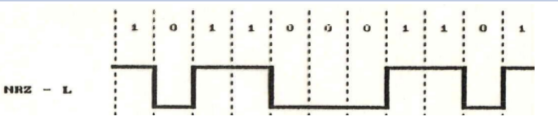
\includegraphics[width=10cm]{img/bande.png}
\end{center}

\begin{description}
  \item[1] : niveau haut
  \item[0] : niveau bas
\end{description}

Logique \textbf{simple} utilisé par les équipements avec une bande passante raisonnable
mais qui a des problèmes de synchronisation.

\subsubsection{Code biphase (Manchester)}

\begin{center}
  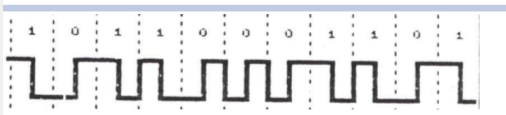
\includegraphics[width=10cm]{img/biphase.png}
\end{center}

\begin{description}
  \item[1] : moitié haut puis moitié bas
  \item[0] : moitié bas puis moitié haut
\end{description}

Nécessite un bit par transition (\textbf{self-clocking}), maximun deux transitions par
bit (\textbf{large bande}) et une détextion d'erreur possible lorsque l'on a une transition
attendue qui est absente.

Utilisé par les bandes magnétiques.

\subsubsection{Code de miller}

\begin{center}
  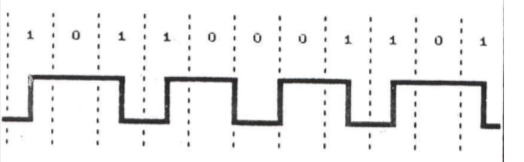
\includegraphics[width=10cm]{img/miller.png}
\end{center}

\begin{description}
  \item[1] : transition en milieu de bit
  \item[01]: rien
  \item[00]: transition après le premier 0
\end{description}

Au moins une transition tout les deux bits et maximum une transition par bit,
une bande de fréquence étroite suffit et une grande sensibilité (càd beaucoup de
configuration possible).

\subsubsection{Autres}

\begin{center}
  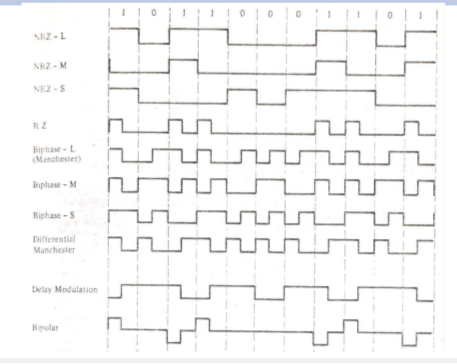
\includegraphics[width=10cm]{img/autres.png}
\end{center}

\newpage
\section{MAC}

\subsection{Support de transmission}
Ligne bifilaire, cable coaxial et fibre optique.

\subsection{Types de réseau}
\subsubsection{Réseau en étoile}
Plusieurs stations connectée à un noeud central.
\begin{itemize}
\item[+] Connexion simple p2p
\item[+] Simplicité des stations extérieures
\item[-] Fragilité : si le noeud cental lache
\end{itemize}

\begin{center}
  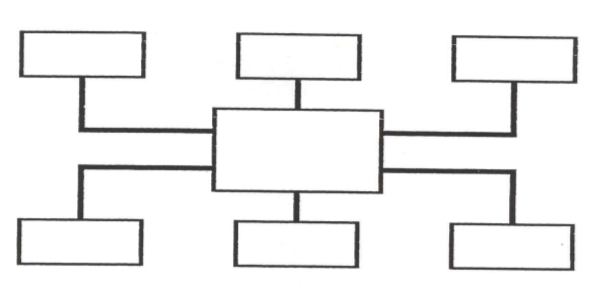
\includegraphics[width=5cm]{img/etoile.png}
\end{center}


\subsubsection{Réseau en anneau}
Chaque station possède un répeteur et les répeteurs sont connecté entre eux de sorte que le réseau forme un cercle avec un seul sens. Chaque répeteur passe le message à son voisin. L’information fait des tours jusqu’a ce que quelqu’un l’enleve du réseau.
\begin{itemize}
\item Difficulté d’insertion de nouvelle station
\item Fragilité: un répeteur lache et bardaf c’est l’embardée
\end{itemize}
Il y a deux types de parades à ces désavantages, les réseau avec anneau double, où les données
transitent dans les deux sens. Avec la possibilité de bloquer des chemins ou de rediriger des flux (voir schéma du cours, j’ai la flemme de dessiner sous latex).

\begin{center}
  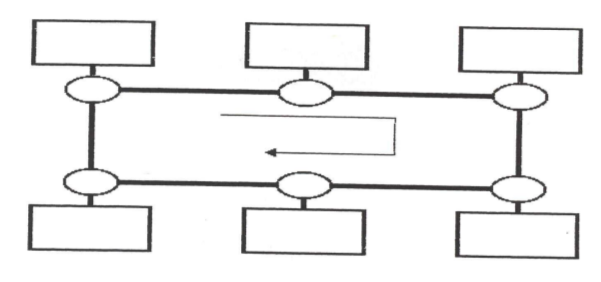
\includegraphics[width=5cm]{img/anneau.png}
\end{center}

\subsubsection{Réseau en bus}
Un bus où toute les stations partagent le même support.

\begin{itemize}
\item[+] Connexion simple de nouvelles stations
\item[+] Gestion plus simplke
\item[+] Pas de fragilité
\item[+] Delai de transmission faible (pas de transition par un intermédiaire)
\item[-] Probl`eme sur le niveau des signaux
\end{itemize}

\begin{center}
  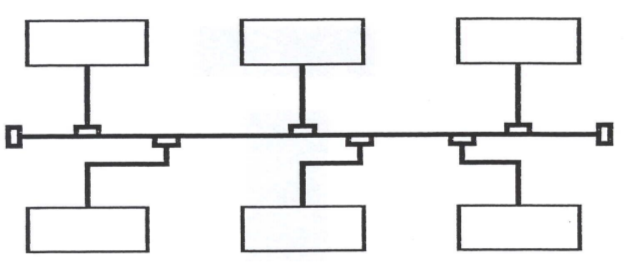
\includegraphics[width=5cm]{img/bus.png}
\end{center}


\subsection{Acces à un réseau}
Dans le multiplexage asynchrone et temporelle, il existe deux types d’acces. Les accès aléatoire et les access déterministe.

\subsubsection{Aléatoire}

\begin{itemize}
\item \textbf{Aloha} On envoi les données sur le bus, si il y a collision avec une autre donnée tu attends un peu avant de renvoyer les données.
\item \textbf{Slotted Aloha} Un Aloha mais avec des cases de données sur le bus. Si deux données se collisionnent elles sont dans la même case (plus efficace que le aloha).
\item \textbf{CSMA} on verifie qu’il n’y a pas de trafic sur le bus et puis on envoi son message
\item \textbf{CSMA/CD} dérivé du système aloha, il s’agit d’un CSMA avec détection des collisions. Dans le système aloha on considère que le temps de communication sur le bus est perdu si deux stations ont parlé dessus en même temps.
\end{itemize}

Il y a plusieurs modes d’access CSMA :
\begin{itemize}
\item \textbf{Persistant} : Si le bus est libre tu emets, sinon tu reregarde le bus
\item \textbf{Non persistant} : Si le bus est libre tu emets, sinon tu attends un peu avant de reessayer
\item \textbf{p-Persistant} : Si le bus est libre tu as une probabilit´e p de pouvoir emettre sinon tu attends. Si le bus n’est pas libre tu r´eessaye sans attendre.
\end{itemize}

\subsubsection{Déterministe}

\begin{itemize}
\item \textbf{Bus à token} : Pour émettre sur un bus on demande l’acces au token. La personne qui a le token parle et les autres la ferme physiquement
\item \textbf{Anneau à token} : le token se ballade sur le réseau et si l’une des stations le voit il peut le récupérer pour parler et devenir le seigneur de l’anneau.
\item \textbf{Evitement de collision} : \textbf{TODO}
\end{itemize}

\subsection{Ethernet}

Ethernet utilise CSMA/CD. Voir schéma du cours pour le format des messages et du token pour
l’ethrnet

\newpage
\section{Questions iCampus}

\subsection{Théorie}

\subsubsection{Qu'est-ce que la pupinisation? Pourquoi n'est-ce plus utilisé?}

La pupinisation consiste à augmenter artificiellement l'impédance de la
ligne en insérant en série des inductances à intervalles réguliers et en créant
un filtre passe-bas pour uniformiser l'inductance électrique de la
ligne. \newline

Cette technique permet de compenser la forte capacité du câble et ainsi
d'améliorer la portée du signal. Ce n'est plus utilisé de nos jours car
cela ne fonctionne que pour les basses fréquences (forte atténuation sur
les hautes fréquences), jusqu'à environ 3.4KHz ce qui limite fortement
la bande passante. Or, ces hautes fréquences sont utilisées par des
technologies comme l'ADSL. \newline

On exprime l'impédance caractéristique d'une ligne comme étant 
$$Z_c = \sqrt{\frac{R + j\omega L}{G + j\omega C}}$$
Et l'on exprime l'exposant de propagation $\gamma$ avec $\alpha$ l'atténuation et $\beta$ le déphasage comme étant
$$\gamma = \sqrt{(R + j\omega L)(G + j\omega C)} = \alpha + j\beta$$

Dans une ligne on suppose G comme étant nul, si dans notre ligne nous
avons la résistance $R$ qui est nettement plus grande que l'inductance
$L$ (cas 1), alors nous avons:
$$\gamma = \sqrt{\frac{\omega RC}{2}} + j\sqrt{\frac{\omega RC}{2}}$$
$$Z_c = \sqrt{\frac{R}{j\omega C}}$$
Nous obtenons donc que l'atténuation et le déphasage sont directement
proportionnels à la fréquence du signal et l'impédance caractéristique
de la ligne qui est inversément proportionnelles à celle-ci (car $\omega
= 2\pi f$). \newline

Si par contre dans notre ligne nous avons la résistance $R$ qui est
nettement plus petite que l'inductance $L$ (cas 2), nous obtenons le résultat suivant:
$$\gamma = \frac{R}{2}\sqrt{\frac{C}{L}} + j\omega \sqrt{LC}$$
$$Z_c = \sqrt{\frac{L}{C}}$$
Ce qui nous donne une impédance et une attenuation indépendante du
signal et un déphasage qui dépend de la fréquence. \newline 

En augmentant artificiellement l'impédance de la ligne (pupinisation)
on évite de se retrouver dans le premier cas. Le second cas correspond à
$\omega L >> R$ qui correspond à celui d'un fil avec peu de résistance et
qui représente une bonne situation pour une ligne.\newline

\subsubsection{Comment caractérise-t-on la directivité d'une antenne? Donnez un
exemple d'application où l'on veut une antenne directive et non directive.}

La directivité d'une antenne est caractérisée par la façon dont elle
rayonne. Si elle rayonne de la même façon dans toutes les directions du
plan horizontal, on dit qu'elle est équidirective et on parle alors
d'antenne isotrope. \newline

Si par contre, elle possède un ou 2 lobes nettement plus importants que
les autres (les lobes principaux), on dit qu'elle est directive. Elle
l'est d'autant plus que le lobe le plus important est étroit
(c'est-à-dire que son angle d'ouverture est petit). \newline

\begin{description}
    \item[Antennes directives] : antennes paraboliques (type Yagi)
    \item[Antennes non directives] : antenne GSM, antenne WiFi
\end{description}

\bigskip

Dans la vie de tous les jours, on préférera avoir une antenne non
directive (avec un angle d'ouverture le plus large possible) lorsque les
stations avec lesquelles on doit communiquer peuvent se déplacer comme
les GSM, les récepteurs WiFi. A contrario, on préfèrera avoir une
antenne directive (avec un angle d'ouverture le plus faible possible)
lorsqu'on sait que l'émetteur et le récepteur ne bougeront pas du jour
au lendemain, on se focalise dans la bonne direction, ce qui permet de
réduire le bruit du signal (comme les antennes paraboliques pour la télévision).

\subsubsection{Décrivez un type de modulation analogique au choix}

\paragraph{La modulation de fréquence}

Cette modulation (FM) consiste à modifier la fréquence du signal à
transmettre en l'augmentant ou la diminuant en fonction de la porteuse.
Si la porteuse (c'est-à-dire la fréquence du signal porteur) est
positive, la fréquence sera augmentée et les sinusoïdes seront plus
rapprochées. \newline

La modulation de fréquence est plus robuste que la modulation
d'amplitude pour transmettre un mesage dans des conditions difficiles
(atténuation et bruit importants).

Exemples d'utilisation :
\begin{itemize}
    \item Les modems bas débit
    \item Les téléphones analogiques
    \item Les radios de la bande FM
    \item Certains synthétiseurs
\end{itemize}

\begin{center}
    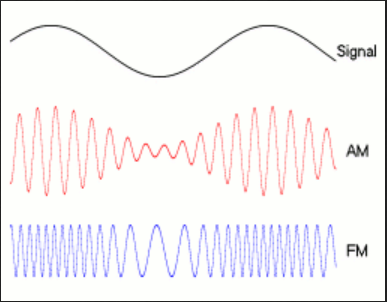
\includegraphics[width=0.5\linewidth]{img/modulation_am_fm.png}
\end{center}

\paragraph{La modulation d'amplitude}

Soit la porteuse $v(t) = A_c cos(\omega_c t + \varphi_c)$, pour avoir une modulation d'amplitude nous allons ajouter le signal \textit{modulant} $m(t)$ multiplié par un \textit{indice de modulation} $k$ à ce signal.
$$s(t) = [1+km(t)] A_c cos(\omega_c t + \varphi_c)$$
Il s'agit donc d'une modulation d'amplitude (AM), ou l'amplitude va
varier en fonction du signal modulant. Il faut bien faire attention dans
le choix de l'indice de modulation (entre 0 et 100\%), pour éviter la surmodulation. En
effet un indice trop élevé pourrait causer un renversement de phase
ce qui pourrait causer de l'ambiguïté lors de la démodulation. \newline

Pour démoduler ce type de modulation on va multiplier le signal modulé par la porteuse (elle doit être disponible à l'émission et à la réception), nous aurons ainsi
\begin{eqnarray*}
A_c s(t)cos(\omega_c t + \varphi_c)*cos(\omega_c t + \varphi_c) &=&A_c s(t)cos^2(\omega_c t + \varphi_c)\\
&=& A_c s(t) \frac{1+ cos(2\omega_c t + 2\varphi_c)}{2}\\
&=& \frac{A_cs(t)}{2} + \frac{A_cs(t)cos(2\omega_c t + 2\varphi_c)}{2}
\end{eqnarray*}
Un filtrage passe bas nous laissera le signal démodulé. \newline

La modulation va aussi créer deux bandes de même taille à gauche et à droite de la porteuse, on voit ca en convertissant le signal du temporel au fréquentiel
$$f(t) cos(\omega_0 t) \Leftrightarrow \frac{F(\omega - \omega_0) + F(\omega + \omega_0)}{2}$$
Dès lors il va falloir choisir combien de bande conserver (en effet il y
a doublon dans l'information). Dès lors plusieurs modes existent :
\begin{itemize}
\item DSB (doubleside band): envoi des deux bandes
\item LSB (lowerside band): on envoi les deux bandes intérieures
\item USB (upperside band): on envoi les deux bandes extérieure
\item QAM (bande latérale unique): on transforme le signal $m(t)$ en
    deux signaux $s_1(t)$ et $s_2(t)$ et l'on envoi $s(t) = s_1(t)
    cos(\omega_c t) + s_2(t) sin(\omega_c t)$. Ainsi une démodulation
    avec $cos(\omega_c t)$ nous fournira $s_1(t)$ et une démodulation
    avec $sin(\omega_c t)$ nous fournira $s_2(t)$. 
\item VSB (vestigialside band): il s'agit d'un envoi en bande latérale
    résiduelle, quand une fréquence est trop près de 0 Hz on ne peut pas
    envoyer une bande latérale unique, on va alors atténuer au maximum
    l'un des cotés.
\end{itemize}

La modulation d'amplitude a un niveau de bruit constant assez élevé. 

\begin{figure}[H]
    \centering
    \begin{minipage}[t]{0.45\linewidth}
        \centering
        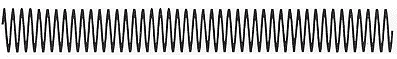
\includegraphics[width=0.75\linewidth]{img/signal_porteur.png}
        \caption{Porteuse (signal porteur)}
    \end{minipage}
    \begin{minipage}[t]{0.45\linewidth}
        \centering
        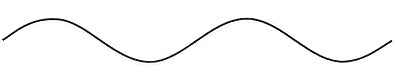
\includegraphics[width=0.75\linewidth]{img/signal_modulant.png}
        \caption{Signal modulant}
    \end{minipage}
\end{figure}

\begin{figure}[H]
    \begin{center}
        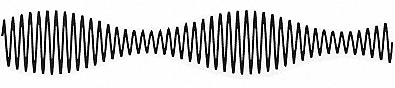
\includegraphics[width=0.335\linewidth]{img/signal_module.png}
        \caption{Signal modulé}
    \end{center}
\end{figure}

\begin{figure}[H]
    \begin{center}
        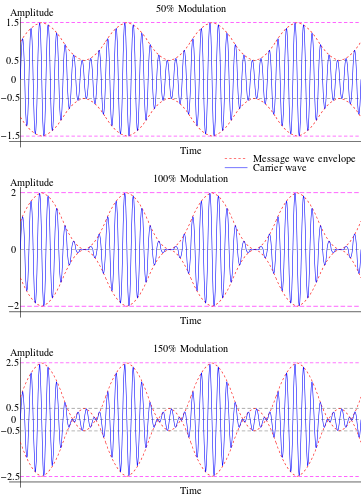
\includegraphics[width=0.5\linewidth]{img/indice_de_modulation_AM.png}
        \caption{Signal modulé selon différents indices de modulation}
    \end{center}
\end{figure}

Comme le démodulateur lit la partie haute du signal, le signal (à cause
de l'indice de modulation trop haut) devient négatif mais le
démodulateur lira un signal positif et disposera alors d'informations
eronnées. \newline

\subsubsection{Décrivez le rôle des différents blocs du schéma de modulation digitale ci dessous.}
\begin{figure}[H]
  \centering
  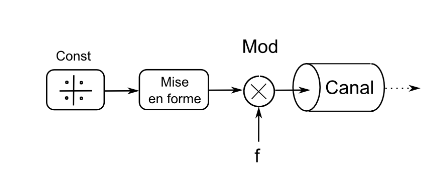
\includegraphics[width=10cm]{img/exo.png}
  \caption{Elements de la modulation digitale}
\end{figure}

\paragraph{Const} ou \textit{mapping du signal}. On transforme
la séquence de bits en séquence de symboles complexes. Il y a 2 axes,
celui des réels (I) et celui des imaginaires (Q). On choisit  ensuite la
constellation suivant le débit voulu, tout en faisant attention au bruit
car la probabilité d'erreurs sur une QAM-16 est plus élevée que sur une
QAM-4. Enfin, si on utilise le mapping de Gray, on veille à ce qu'il n'y
ait qu'un seul bit de différence entre les points les + proches.
\newline

\begin{figure}[H]
    \centering
    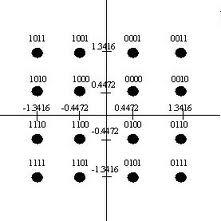
\includegraphics[width=0.5\linewidth]{img/mapping.png}
    \caption{Exemple de mapping}
\end{figure}

\paragraph{Mise en forme} Grâce au passage par Const, on sait que le
nombre d'inputs possibles est fini, assurant qu'on peut assigner à
chaque input une certaine valeur sous forme de courant pour créer le
signal. Chaque input sera transmis pendant un intervalle de temps T qui
correspond à la fréquence d'échantillonage.
Cette mise en forme est rectangulaire (une certaine tension pendant
une certaine durée) et \og{}abrupte\fg{} puisqu'elle provoque
des passages de courant de +1V à -1V instantanément (irréalisable en
pratique). En pratique, le passage entre les différentes tensions se
fait sur une durée plus longue, ceci peut provoquer l'ISI (Inter Symbol
Interference) qui consiste à l'incompréhension du signal par le
récepteur. Pour éviter cette situation, on applique le critère de
Nyquist qui consiste à échantilloner au milieu du moment (chaque T/2) où le signal a
été envoyé, qui correspond normalement à l'endroit qui a le plus de
chance de contenir la valeur que l'émetteur souhaitait transmettre. Pour
que ce critère fonctionne, il faut une bonne synchronisation entre
l'émetteur et le récepteur, que la mise en forme respecte le principe de
superposition (c'est-à-dire soit linéaire : la somme de deux entrées
quelconques égale à la somme de deux sorties quelconques ; le multiple
d'une entrée quelconque correspond au multiple de la sortie
correspondante) ainsi que peu de dispersion sur le signal.\newline

On peut décider de garder une seule partie du signal grâce à un filtre
passe-bas (garder les basses fréquences), un filtre passe-haut (garder
les hautes fréquences) ou un filtre passe bande (garder une certaine
bande de fréquence). \newline

\paragraph{Modulateur de fréquence}

La modulation (FM) consiste à modifier la fréquence du signal à
transmettre en l'augmentant ou la diminuant en fonction de la porteuse.
Si la porteuse (c'est-à-dire la fréquence du signal porteur) est
positive, la fréquence sera augmentée et les sinusoïdes seront plus
rapprochées. \newline

La modulation de fréquence est plus robuste que la modulation
d'amplitude pour transmettre un mesage dans des conditions difficiles
(atténuation et bruit importants).

Exemples d'utilisation :
\begin{itemize}
    \item Les modems bas débit
    \item Les téléphones analogiques
    \item Les radios de la bande FM
    \item Certains synthétiseurs
\end{itemize}

\begin{center}
    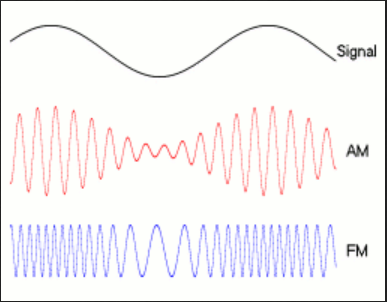
\includegraphics[width=0.5\linewidth]{img/modulation_am_fm.png}
\end{center}


\subsubsection{Quel est le principe du CDMA ? Deux exemples d'options alternatives pour
implémenter la division de l'accès pour les différents utilisateurs.}

Le CDMA (code division multiple access) attribue un code (une sorte
d'identifiant) à chaque personne qui communique sur le canal pour lui
permettre de communiquer simultanément sur la même fréquence porteuse.
Chaque code est différent et il y a une très faible corrélation entre
les différents codes, ce qui permet à l'émetteur de créer un seul signal
qui contient les informations pour tous les utilisateurs et aux
utilisateurs de décoder ce signal en faisant une multiplication avec
leur code. Ce mécanisme fonctionne très bien quand il y a peu
d'utilisateurs sur le réseau et il permet à chacun de profiter de la
totalité de la bande passante.\newline

Une première alternative est le TDMA qui divise la bande passante en
un ensemble de timeslot que les différents utilisateurs vont pouvoir
utiliser, ce qui limite l'usage de chaque utilisateur à un certain
temps. Cette technique est un multiplexage temporel où la même fréquence
est attribuée à différents utilisateurs qui se partagent le temps selon
les time slices.\newline

Une seconde alternative est le FDMA qui permet de séparer le canal en un ensemble de canaux de
fréquence indépendants. Il faut faire attention dans ce type de
multiplexage que les canaux soit bien séparé. Chaque utilisateur a donc
une bande de fréquence différente.\newline

\begin{figure}[H]
    \centering
    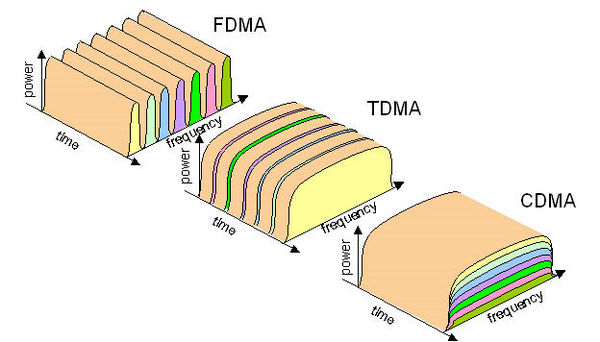
\includegraphics[width=0.65\linewidth]{img/fdma_tdma_cdma.png}
    \caption{Différence entre le FDMA, TDMA et CDMA}
\end{figure}

\subsubsection{Qu'est-ce que le mécanisme ARQ? Pourquoi est il parfois
    utilisé à la place des correcteurs d'erreurs et quand ?}

Le mécanisme ARQ est un mécanisme de contrôle d'erreurs utilisé quand on
désire une plus grande fiabilité dans les communications. Il se base sur
des acquittements (ACK) envoyés du récepteur à l'émetteur.
Il s'agit d'un système de transmission de
données appartenant à la couche Liaison (niveau 2) du modèle OSI. Il
existe plusieurs modes à ce système de transmission.
\begin{itemize}
\item \textbf{Stop-and-wait} A chaque paquet de données envoyé
    l'émetteur attend une confirmation (ACK) du récepteur. Si il y a une
    erreur, l'émetteur renvoie le paquet. 
\item \textbf{Go-back-n} L'émetteur envoie un certain nombre de ses paquets sans attendre la
    réponse de l'utilisateur. S'il reçoit sur un acquittement contenant un
    nombre ne correspondant pas à celui de la dernière trame envoyée, ce
    nombre identifie le premier paquet manquant et l'émetteur redémarre l'envoi à partir de
    celui-ci. Dès que le récepteur voit une
    erreur il arrête de récupérer des paquets.
\item \textbf{Selective-repeat} Lorsqu'une erreur intervient le
    récepteur prévient l'émetteur en lui disant quel paquet a foiré,
    mais il continue à récuperer les paquets. A un moment l'emetteur va
    renvoyer le paquet manquant en question.
\end{itemize}

\begin{figure}[H]
    \centering
    \begin{minipage}[t]{0.3\linewidth}
        \centering
        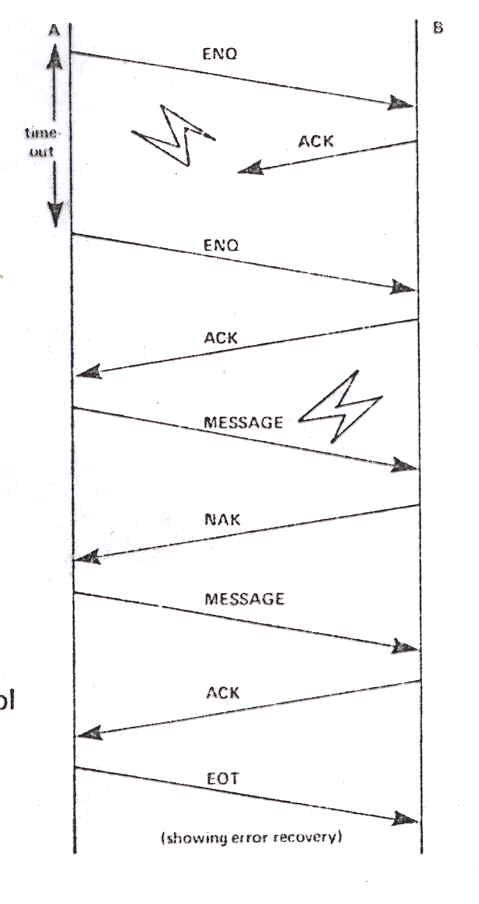
\includegraphics[width=\linewidth]{img/stop_and_wait.png}
        \caption{Stop and wait}
    \end{minipage}
    \begin{minipage}[b]{0.6\linewidth}
        \centering
        \begin{minipage}[t]{\linewidth}
            \centering
            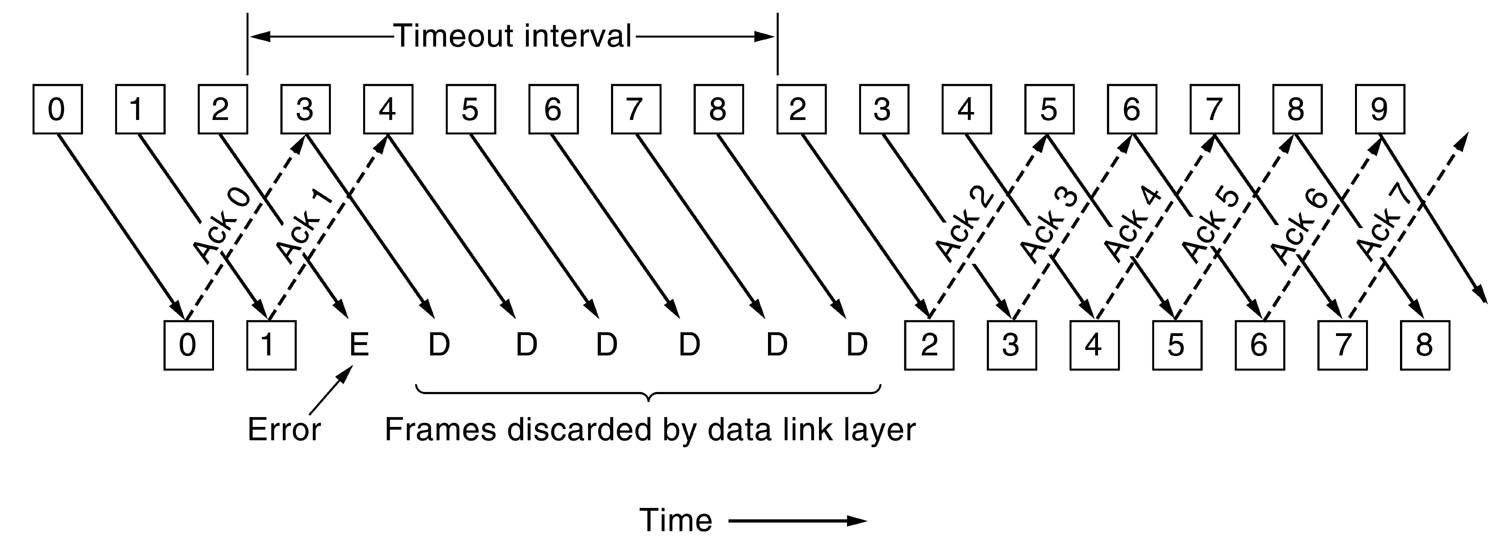
\includegraphics[width=\linewidth]{img/go_back_n.png}
            \caption{Go-back-n}
        \end{minipage}
        \begin{minipage}[b]{\linewidth}
            \centering
            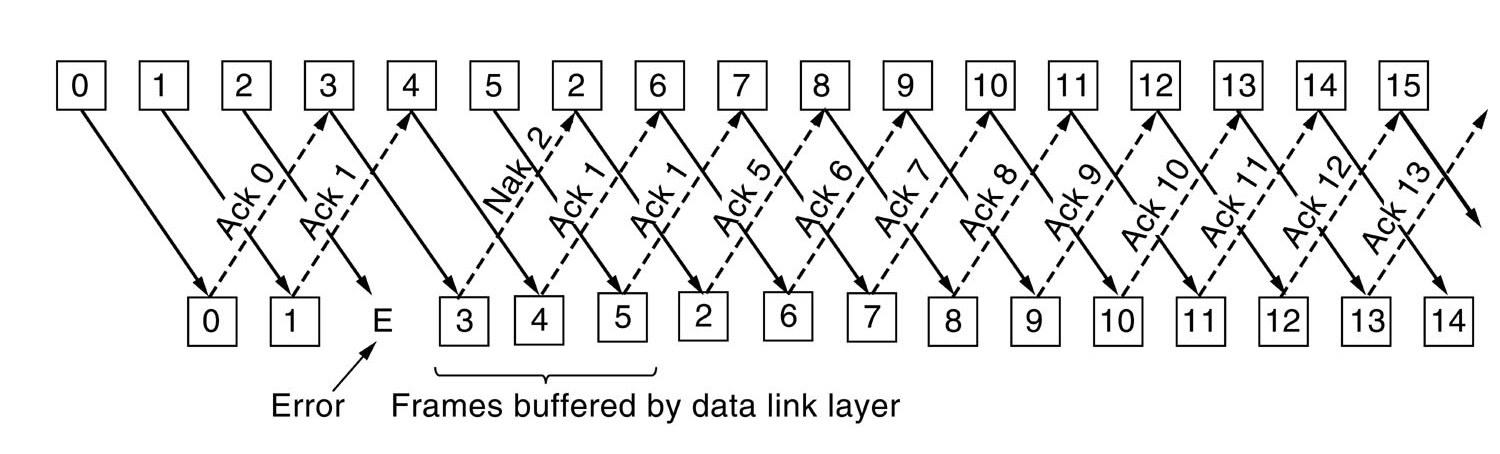
\includegraphics[width=\linewidth]{img/selective_repeat.png}
            \caption{Selective repeat}
        \end{minipage}
    \end{minipage}
\end{figure}

Le mécanisme ARQ est utilisé parfois à
la place des codes correcteurs d'erreurs tout simplement parce que dans
certains cas utiliser un code correcteur d'erreurs est simplement trop
couteux. En effet, supposons que l'on veut envoyer $10^6$ bits par
blocs de 1000bits. Si on a une ligne T1 de transmission avec un taux d'erreur (BER) de
$10^{-6}$ (sur 1 millions de bit, il y en un seul fautif)
et une ligne T2 avec un taux d'erreur de $10^{-4}$. \\
Si on utilise un code(1010,1000) pour corriger les erreurs simples. On a
besoin de 10000 bits de contrôle (car on a 1000 blocs)
cela pour T1 et T2.

Par contre si utilise un code(1001,1000) pour détecter les erreurs (par exemple la parité):
\begin{itemize}
\item Dans T1,  pour les 1000 blocs, on aura envoyé les 1000 bits de
    contrôle + la répétition des 1001 bits du blocs qui contient le bit
    eronné, on a donc ajouté 2001 bits (raisonnable).
\item Dans T2, on aura aussi envoyé 1000 bits de contrôle mais en plus
    la répétiion des 100*10001 bits des blocs erronés (le 100 vient du fait que sur les $10^6$ bits il y en a 100 fautifs). On aura donc ajouter en tout avec notre code détecteurs d'erreurs plus de 100 000 bits.
\end{itemize}

En conclusion, si le taux d'erreur est faible, il est plus intéressant
de renvoyer un paquet de temps en temps plutôt que d'ajouter énormément
de répétition pour s'assurer de la reconstruction des paquets en cas
d'erreur. \newline

\subsubsection{Quel est l'interêt de la DCT dans le codage JPEG? La DCT est elle une
opération avec ou sans pertes ?}

La DCT est une transformée de Fourier avec cosinus qui permet de
remplacer une matrice $8\times 8$ pixels contenant de la luminance en
une matrice de $8\times 8$ coefficients DCT contenant exactement la même
information. Cette application de Fourier est sans pertes, cependant son
intérêt réside dans le fait que certains coefficients sont moins
importants que d'autres. \newline

Il s'agit des coefficients à hautes fréquences
(situés en haut à gauche de la matrice) qui sont réservés à des
changements rapides d'intensité du pixel (contraste élevé), généralement invisible à
l'\oe il nu. On peut omettre certains de ces coefficients sans risquer
une grosse perte de qualité pour l'\oe il humain, ce qui
permet de faire une compression, celle-ci se fait donc avec pertes
puisqu'on ne pourra jamais retrouver les coefficients négligés.

\subsubsection{Qu'est-ce que l'alignement temporel dans le système GSM? Pourquoi
est-il seulement nécessaire dans la liaison montante?}

Le système GSM utilise la technologie TDMA, cette technologie consiste à
allouer à chaque utilisateur un time slot particulier lors duquel il
peut utiliser la fréquence. Lorsqu'un utilisateur passe un appel avec
son GSM, il peut se déplacer et donc changer sa distance par rapport à
l'antenne, changeant ainsi le temps qu'il met à la joindre par onde. Ce
changement de distance (et de délai) peut provoquer un overlap des time
slots alloués aux utilisateurs créant ainsi des interférences.\newline

Pour éviter cette situation, on a introduit l'alignement temporel qui
consiste à adapter la réception en faisant un décalage de bits pour
rester dans le bon timeslot. C'est uniquement nécessaire dans la liaison
montante car c'est le GSM qui fait le décalage, pas l'antenne. \newline

\subsubsection{Qu'est-ce qu'un algorithme de cryptographique à clé publique?
Dans quel cadre est-il généralement utilisé? Quels sont ses désavantages?}

Un algorithme à clé publique (ou asymétrique) correspond à un algorithme
de cryptographie utilisant 2 types de clés. \newline

Supposons A et B, deux personnes souhaitant s'envoyer des messages dont
ils souhaitent garder le contenu secret. Les messages vont être cryptées
mathématiquement par des fonctions à sens unique, telles qu'elles
nécessitent les informations de deux clés pour retrouver la formule à
partir de la solution. Parmi ces deux clés, A va en garder une secrète
(c'est une clé privée) et va en envoyer une à B. B va crypter ses
messages à l'aide de la clé publique, les rendant lisible uniquement par
quelqu'un qui aurait la \og{}clé publique\fg{}, sorte de brèche secrète
de l'équation. De cette manière, quelqu'un qui intercepterait la clé
publique et/ou les messages entre A et B serait incapable de les
comprendre sans avoir accès à la clé privée.\newline

Ce chiffrement est plus lent, plus difficile et les clés doivent être plus
longues pour assurer un même niveau de sécurité qu'avec la cryptographie
symétrique. La véritable difficulté est d'être sûr que le créateur de la
clé publique n'est pas un utilisateur autre que A (malveillant) qui
l'aurait communiqué à B, ce qui demande des certifications de clés
publiques. \newline

\begin{figure}[H]
    \centering
    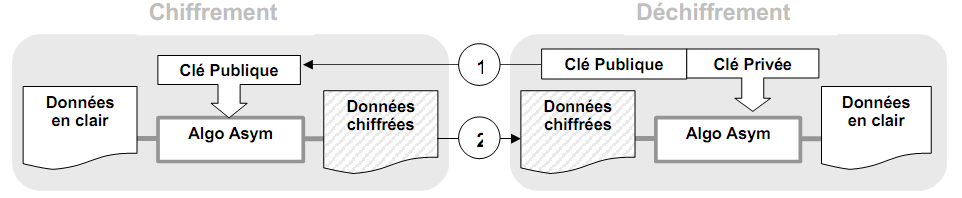
\includegraphics[width=\linewidth]{img/algorithme_asymetrique.png}
    \caption{Schéma d'utilisation d'un algorithme asymétrique}
\end{figure}

\subsubsection{Qu'est-ce la distorsion et à quoi est-ce dû ?}

La distorsion (ou \textit{dispersion}) correspond à une des
caractéristiques des lignes, c'est l'ensemble des modifications
indésirables d'un signal (sauf gain/atténuation/retard). \newline

Concrètement, il s'agit d'une déformation non-linéaire d'un signal (majoritairement
les signaux analogiques) qui peut être par exemple provoqué par la
présence d'une harmonique (le plus souvent une harmonique de rang 3) qui
s'ajoute au signal. Comme un signal peut toujours se décomposer en une
somme de sinusoïde, la troisième harmonique et le signal de base vont
constituer un nouveau signal qui ne permettra pas de retrouver le signal
original. \newline

\begin{figure}[H]
    \centering
    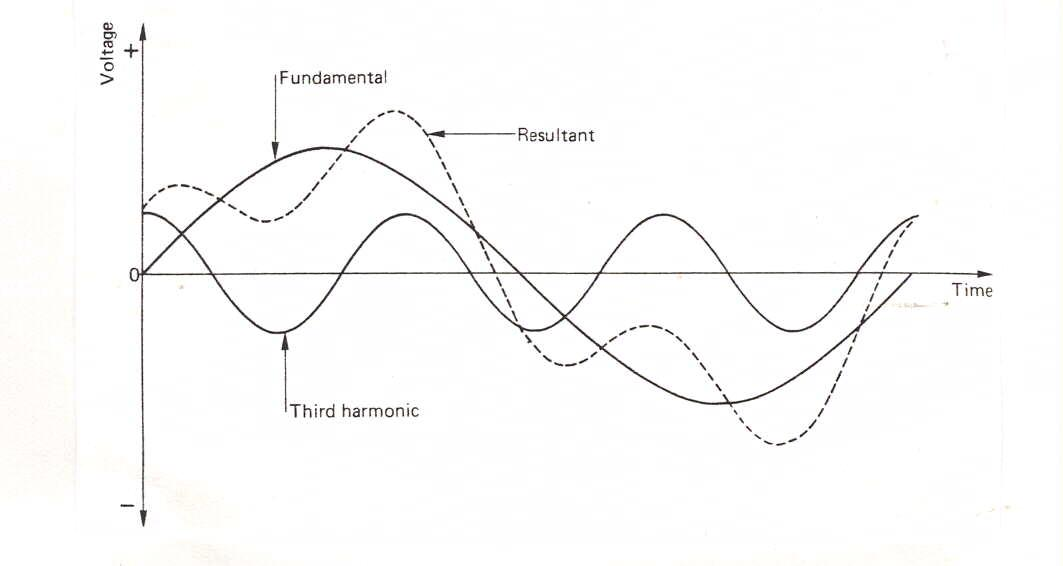
\includegraphics[width=0.7\linewidth]{img/dispersion.png}
    \caption{Exemple de dispersion}
\end{figure}

\subsubsection{Qu'est-ce que l'atténuation et à quoi est-ce dû ?}

L'atténuation est la diminution de l'amplitude ou de la puissance d'un
signal lors de sa transmission. Elle est dûe à la distance (la puissance
d'un signal diminue de manière exponentielle) et est donc un facteur
limitatif dans les télécommunications. \newline

Idée :
\[
    \textrm{Atténuation} = \frac{\textrm{valeur en
    sortie}}{\textrm{valeur en entrée}}
\]
\bigskip

Calcul en décibels :
\[ p_1 \textrm{: la puissance en entrée} \]
\[ p_2 \textrm{: la puissance en sortie} \]
\[ P = U.I \]
\[ U = R.I \]
\[ P = \frac{U^{2}}{R} \]
\[
    10 log(\frac{p_1}{p_2}) = 10 log(\frac{u_1^2}{u_2^2}) = 20
    log(\frac{u_1}{u_2})
\]

Coefficient d'atténuation $\alpha$ : 
\[ \bm{\alpha} [dB/(MHz \times cm)] =
\frac{\bm{Atténuation} [dB]}{\mathbf{l} [cm] \cdot \mathbf{f} [MHz]} \]

\subsubsection{Expliquer la création de l'image pour une télévision
analogique.}

La télévision utilise la bande de fréquence compris entre 40 et 70 MHz.
Pour capturer l'image, on utilise le dispositif optique d'une caméra
et un microphone (dispositifs analogiques). Le matériel pour les
captations ont des limites fixées dans lesquelles varient le courant et
la tension électrique de manière continue. Les signaux analogiques sont
ensuite transformés en signaux numériques avant d'être envoyés à un
récepteur (numérisation et modulation). \newline

Pour afficher l'image sur une télévision cathodique, on utilise 2 trames
qui utilisent chacune 2 fields. Chaque trame construit une moitié de
l'image, chaque field construit une moitié de ligne. \newline

Chaque pixel de l'image est consistué d'un nombre fini d'informations
sous la forme (Red,Green,Blue) les couleurs qui permettent elles-mêmes de retrouver
(Y,U,V) la luminance et les chrominances. \newline

\subsubsection{En quoi consiste le bruit ?}

Le bruit est une partie d'un signal qui ne transporte pas d'information
ou transporte une information indésirable. C'est une sorte de signal
aléatoire qu'on ne peut pas décoder. \newline 

Les circuits numériques limitent l'impact du bruit, cependant il est
présent en particulier dans les petits composants à faible tension et à
fréquence élevée (glitches). Les circuits analogiques subissent le bruit
comme un dysfonctionnement passager ou une dégradation des performances.
\newline

\subsubsection{En quoi consiste le multiplexage ?}

Il existe deux types de multiplexage : le multiplexage temporel et le
multiplexage fréquentiel. \newline

Le \textbf{multiplexage fréquentiel} consiste à allouer des fractions de
la bande passante à chaque communication. Exemple : FDMA \newline

Le \textbf{multiplexage temporel} consiste à répartir le temps
d'utilisation de la totalité de la bande passante entre les différentes
communications. Exemple : TDMA\newline

\subsubsection{En quoi consiste la quantification ?}

La quantification est un procédé qui permet d'approcher un signal
continu par les valeurs d'un ensemble discret d'assez petite taille.
C'est utilisé pour faire de la conversion analogique-numérique mais
également pour la compression des signaux audio et des images. 

\subsubsection{Expliquer le principe de la réception superhétérodyne.}

\begin{figure}[H]
    \centering
    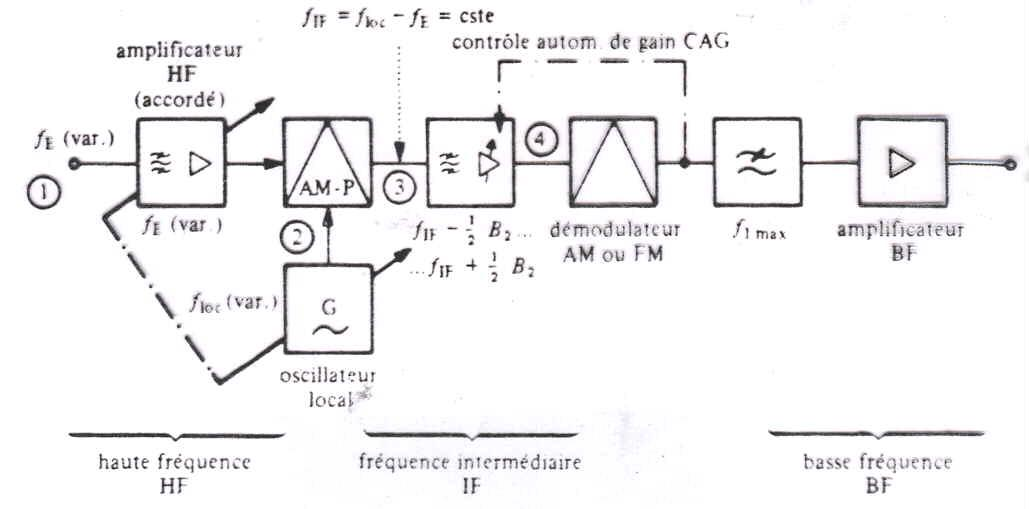
\includegraphics[width=\linewidth]{img/reception_superheterodyne.png}
    \caption{Schéma récapitulatif de la réception superhétérodyne}
\end{figure}

On reçoit un signal qui contient la fréquence sur laquelle on doit se
caler (1). Un amplificateur HF (haute fréquence) assure une première
amplification du signal (suppression du bruit utile pour les fréquences
élevées). Avec le signal provenant de l'oscillateur (2) et celui provenant
de l'antenne, on produit un signal modulé en amplitude (3). Le signal passe
ensuite dans un filtre de fréquence intermédiaire qui va supprimer
certaines composantes non-nécessaires du signal produites lors du
passage par l'étape précédente. Le signal passe par un amplificateur
responsable du gain qui contient aussi un contrôle automatique du gain
(CAG).  \newline

Le nouveau signal (4) est maintenant à un niveau nécessaire pour la
démodulation (d'amplitude ou de fréquence). Les fréquences indésirables
sont filtrées à la sortie de l'amplificateur. Le signal passe enfin par
un amplificateur basse fréquence. \newline

\subsubsection{Expliquer les principes du codage de Vernam}

Le codage de Vernam est une technique de cryptographie qui consiste à
chiffrer avec un message \og{}en clair\fg{} avec une clé présentant
certaines caractéristiques :

\begin{enumerate}
    \item La clé doit être une suite de caractères aussi longue que le
        message à chiffrer.
    \item Les caractères composant la clé doivent être choisis de façon
        totalement aléatoire.
    \item Chaque clé ne doit être utilisée qu'une seule fois (jetable)
\end{enumerate}

Si on respecte ces règles, le système offre une sécurité absolue.
L'envoyeur et le récepteur du message doivent posséder la clé et pour la
transmission de cette clé de manière totalement sûr, elle doit être
physique. Le problème de la sécurité se passe est donc physique, les
applications sont surtout militaires.
\newline

\subsubsection{En quoi consiste l'échantillonnage ?}

L'échantillonnage consiste à transmettre un signal en capturant des
valeurs à intervalles réguliers. Il produit une suite de valeurs
discrètes. Il s'utilise dans le cadre d'une numérisation d'un signal. 

\subsubsection{En quoi consiste la numérisation ?}

La numérisation est la conversion d'un signal analogique (continu)
en un signal numérique (discret). \newline

La numérisation se fait en plusieurs étapes :
\begin{enumerate}
    \item L'\textbf{échantillonnage} prélève à intervalles réguliers des valeurs
        du signal.
    \item La \textbf{quantification} transforme une valeur quelconque en une
        valeur prise dans une liste finie de valeurs valides pour le
        système.
    \item Le \textbf{codage} fait correspondre à chaque valeur valide pour le
        système un code numérique.
\end{enumerate}

Les avantages sont nombreux : ça permet un traitement informatique des
données (les ordinateurs ne peuvent traiter que des formes discrètes),
le stockage des signaux et donc leur re-création et la possibilité
d'appliquer des codes détecteurs (voire correcteurs) sur ceux-ci.
\newline

\subsubsection{Expliquez le mécanisme de démodulation d'un signal}

\begin{figure}[H]
% Schéma d'un démodulateur en tikz
\ifx\du\undefined
  \newlength{\du}
\fi
\setlength{\du}{15\unitlength}
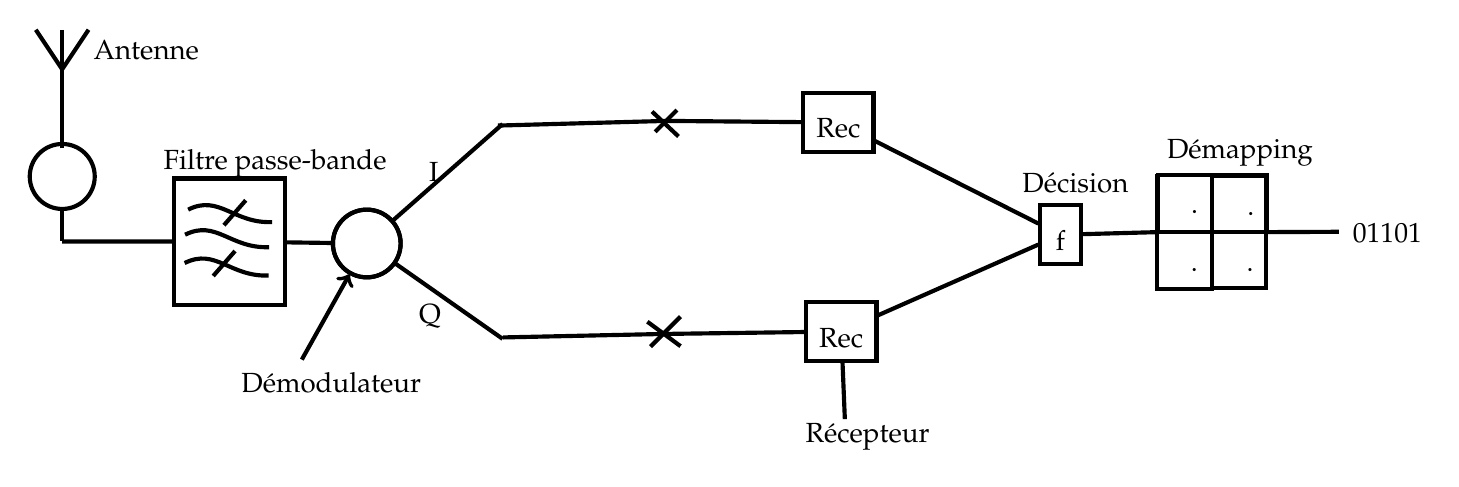
\begin{tikzpicture}[scale=0.75]
\pgftransformxscale{1.000000}
\pgftransformyscale{-1.000000}
\definecolor{dialinecolor}{rgb}{0.000000, 0.000000, 0.000000}
\pgfsetstrokecolor{dialinecolor}
\definecolor{dialinecolor}{rgb}{1.000000, 1.000000, 1.000000}
\pgfsetfillcolor{dialinecolor}
\pgfsetlinewidth{0.100000\du}
\pgfsetdash{}{0pt}
\pgfsetdash{}{0pt}
\pgfsetbuttcap
\pgfsetmiterjoin
\pgfsetlinewidth{0.100000\du}
\pgfsetbuttcap
\pgfsetmiterjoin
\pgfsetdash{}{0pt}
\definecolor{dialinecolor}{rgb}{0.000000, 0.000000, 0.000000}
\pgfsetstrokecolor{dialinecolor}
\draw (7.102782\du,6.662500\du)--(7.102782\du,4.120833\du);
\pgfsetbuttcap
\pgfsetmiterjoin
\pgfsetdash{}{0pt}
\definecolor{dialinecolor}{rgb}{0.000000, 0.000000, 0.000000}
\pgfsetstrokecolor{dialinecolor}
\draw (6.255560\du,2.850000\du)--(7.102782\du,4.120833\du);
\pgfsetbuttcap
\pgfsetmiterjoin
\pgfsetdash{}{0pt}
\definecolor{dialinecolor}{rgb}{0.000000, 0.000000, 0.000000}
\pgfsetstrokecolor{dialinecolor}
\draw (7.102782\du,2.850000\du)--(7.102782\du,4.120833\du);
\pgfsetbuttcap
\pgfsetmiterjoin
\pgfsetdash{}{0pt}
\definecolor{dialinecolor}{rgb}{0.000000, 0.000000, 0.000000}
\pgfsetstrokecolor{dialinecolor}
\draw (7.950004\du,2.850000\du)--(7.102782\du,4.120833\du);
\pgfsetlinewidth{0.100000\du}
\pgfsetdash{}{0pt}
\pgfsetdash{}{0pt}
\pgfsetbuttcap
\pgfsetmiterjoin
\pgfsetlinewidth{0.100000\du}
\pgfsetbuttcap
\pgfsetmiterjoin
\pgfsetdash{}{0pt}
\definecolor{dialinecolor}{rgb}{0.000000, 0.000000, 0.000000}
\pgfsetstrokecolor{dialinecolor}
\pgfpathellipse{\pgfpoint{7.106250\du}{7.562500\du}}{\pgfpoint{1.043750\du}{0\du}}{\pgfpoint{0\du}{1.043750\du}}
\pgfusepath{stroke}
\pgfsetbuttcap
\pgfsetmiterjoin
\pgfsetdash{}{0pt}
\definecolor{dialinecolor}{rgb}{0.000000, 0.000000, 0.000000}
\pgfsetstrokecolor{dialinecolor}
\draw (7.106250\du,6.518750\du)--(7.106250\du,5.475000\du);
\pgfsetbuttcap
\pgfsetmiterjoin
\pgfsetdash{}{0pt}
\definecolor{dialinecolor}{rgb}{0.000000, 0.000000, 0.000000}
\pgfsetstrokecolor{dialinecolor}
\draw (7.106250\du,8.606250\du)--(7.106250\du,9.650000\du);
\definecolor{dialinecolor}{rgb}{1.000000, 1.000000, 1.000000}
\pgfsetfillcolor{dialinecolor}
\fill (10.700000\du,7.627740\du)--(10.700000\du,11.677740\du)--(14.250000\du,11.677740\du)--(14.250000\du,7.627740\du)--cycle;
\pgfsetlinewidth{0.100000\du}
\pgfsetdash{}{0pt}
\pgfsetdash{}{0pt}
\pgfsetmiterjoin
\definecolor{dialinecolor}{rgb}{0.000000, 0.000000, 0.000000}
\pgfsetstrokecolor{dialinecolor}
\draw (10.700000\du,7.627740\du)--(10.700000\du,11.677740\du)--(14.250000\du,11.677740\du)--(14.250000\du,7.627740\du)--cycle;
% setfont left to latex
\definecolor{dialinecolor}{rgb}{0.000000, 0.000000, 0.000000}
\pgfsetstrokecolor{dialinecolor}
\node at (12.475000\du,9.847740\du){};
\pgfsetlinewidth{0.100000\du}
\pgfsetdash{}{0pt}
\pgfsetdash{}{0pt}
\pgfsetbuttcap
{
\definecolor{dialinecolor}{rgb}{0.000000, 0.000000, 0.000000}
\pgfsetfillcolor{dialinecolor}
% was here!!!
\definecolor{dialinecolor}{rgb}{0.000000, 0.000000, 0.000000}
\pgfsetstrokecolor{dialinecolor}
\draw (7.106250\du,9.650000\du)--(10.649809\du,9.651808\du);
}
\pgfsetlinewidth{0.100000\du}
\pgfsetdash{}{0pt}
\pgfsetdash{}{0pt}
\pgfsetmiterjoin
\pgfsetbuttcap
{
\definecolor{dialinecolor}{rgb}{0.000000, 0.000000, 0.000000}
\pgfsetfillcolor{dialinecolor}
% was here!!!
\definecolor{dialinecolor}{rgb}{0.000000, 0.000000, 0.000000}
\pgfsetstrokecolor{dialinecolor}
\pgfpathmoveto{\pgfpoint{11.150000\du}{8.627740\du}}
\pgfpathcurveto{\pgfpoint{12.150000\du}{8.127740\du}}{\pgfpoint{12.600000\du}{9.077740\du}}{\pgfpoint{13.850000\du}{9.027740\du}}
\pgfusepath{stroke}
}
\pgfsetlinewidth{0.100000\du}
\pgfsetdash{}{0pt}
\pgfsetdash{}{0pt}
\pgfsetmiterjoin
\pgfsetbuttcap
{
\definecolor{dialinecolor}{rgb}{0.000000, 0.000000, 0.000000}
\pgfsetfillcolor{dialinecolor}
% was here!!!
\definecolor{dialinecolor}{rgb}{0.000000, 0.000000, 0.000000}
\pgfsetstrokecolor{dialinecolor}
\pgfpathmoveto{\pgfpoint{11.052100\du}{9.433590\du}}
\pgfpathcurveto{\pgfpoint{12.052100\du}{8.933590\du}}{\pgfpoint{12.502100\du}{9.883590\du}}{\pgfpoint{13.752100\du}{9.833590\du}}
\pgfusepath{stroke}
}
\pgfsetlinewidth{0.100000\du}
\pgfsetdash{}{0pt}
\pgfsetdash{}{0pt}
\pgfsetmiterjoin
\pgfsetbuttcap
{
\definecolor{dialinecolor}{rgb}{0.000000, 0.000000, 0.000000}
\pgfsetfillcolor{dialinecolor}
% was here!!!
\definecolor{dialinecolor}{rgb}{0.000000, 0.000000, 0.000000}
\pgfsetstrokecolor{dialinecolor}
\pgfpathmoveto{\pgfpoint{11.037100\du}{10.343600\du}}
\pgfpathcurveto{\pgfpoint{12.037100\du}{9.843590\du}}{\pgfpoint{12.487100\du}{10.793600\du}}{\pgfpoint{13.737100\du}{10.743600\du}}
\pgfusepath{stroke}
}
\pgfsetlinewidth{0.100000\du}
\pgfsetdash{}{0pt}
\pgfsetdash{}{0pt}
\pgfsetbuttcap
{
\definecolor{dialinecolor}{rgb}{0.000000, 0.000000, 0.000000}
\pgfsetfillcolor{dialinecolor}
% was here!!!
\definecolor{dialinecolor}{rgb}{0.000000, 0.000000, 0.000000}
\pgfsetstrokecolor{dialinecolor}
\draw (13.000000\du,8.327740\du)--(12.300000\du,9.127740\du);
}
\pgfsetlinewidth{0.100000\du}
\pgfsetdash{}{0pt}
\pgfsetdash{}{0pt}
\pgfsetbuttcap
{
\definecolor{dialinecolor}{rgb}{0.000000, 0.000000, 0.000000}
\pgfsetfillcolor{dialinecolor}
% was here!!!
\definecolor{dialinecolor}{rgb}{0.000000, 0.000000, 0.000000}
\pgfsetstrokecolor{dialinecolor}
\draw (12.655600\du,9.958290\du)--(11.955600\du,10.758300\du);
}
\pgfsetlinewidth{0.100000\du}
\pgfsetdash{}{0pt}
\pgfsetdash{}{0pt}
\pgfsetbuttcap
\pgfsetmiterjoin
\pgfsetlinewidth{0.100000\du}
\pgfsetbuttcap
\pgfsetmiterjoin
\pgfsetdash{}{0pt}
\definecolor{dialinecolor}{rgb}{1.000000, 1.000000, 1.000000}
\pgfsetfillcolor{dialinecolor}
\pgfpathellipse{\pgfpoint{16.887500\du}{9.715240\du}}{\pgfpoint{1.087500\du}{0\du}}{\pgfpoint{0\du}{1.087500\du}}
\pgfusepath{fill}
\definecolor{dialinecolor}{rgb}{0.000000, 0.000000, 0.000000}
\pgfsetstrokecolor{dialinecolor}
\pgfpathellipse{\pgfpoint{16.887500\du}{9.715240\du}}{\pgfpoint{1.087500\du}{0\du}}{\pgfpoint{0\du}{1.087500\du}}
\pgfusepath{stroke}
\pgfsetbuttcap
\pgfsetmiterjoin
\pgfsetdash{}{0pt}
\definecolor{dialinecolor}{rgb}{0.000000, 0.000000, 0.000000}
\pgfsetstrokecolor{dialinecolor}
\pgfpathellipse{\pgfpoint{16.887500\du}{9.715240\du}}{\pgfpoint{1.087500\du}{0\du}}{\pgfpoint{0\du}{1.087500\du}}
\pgfusepath{stroke}
\pgfsetlinewidth{0.100000\du}
\pgfsetdash{}{0pt}
\pgfsetdash{}{0pt}
\pgfsetbuttcap
{
\definecolor{dialinecolor}{rgb}{0.000000, 0.000000, 0.000000}
\pgfsetfillcolor{dialinecolor}
% was here!!!
\definecolor{dialinecolor}{rgb}{0.000000, 0.000000, 0.000000}
\pgfsetstrokecolor{dialinecolor}
\draw (14.300435\du,9.678596\du)--(15.767139\du,9.699371\du);
}
\pgfsetlinewidth{0.100000\du}
\pgfsetdash{}{0pt}
\pgfsetdash{}{0pt}
\pgfsetbuttcap
{
\definecolor{dialinecolor}{rgb}{0.000000, 0.000000, 0.000000}
\pgfsetfillcolor{dialinecolor}
% was here!!!
\definecolor{dialinecolor}{rgb}{0.000000, 0.000000, 0.000000}
\pgfsetstrokecolor{dialinecolor}
\draw (17.740616\du,8.964791\du)--(21.250000\du,5.877740\du);
}
\pgfsetlinewidth{0.100000\du}
\pgfsetdash{}{0pt}
\pgfsetdash{}{0pt}
\pgfsetbuttcap
{
\definecolor{dialinecolor}{rgb}{0.000000, 0.000000, 0.000000}
\pgfsetfillcolor{dialinecolor}
% was here!!!
\definecolor{dialinecolor}{rgb}{0.000000, 0.000000, 0.000000}
\pgfsetstrokecolor{dialinecolor}
\draw (17.818632\du,10.368891\du)--(21.250000\du,12.777700\du);
}
\pgfsetlinewidth{0.100000\du}
\pgfsetdash{}{0pt}
\pgfsetdash{}{0pt}
\pgfsetbuttcap
{
\definecolor{dialinecolor}{rgb}{0.000000, 0.000000, 0.000000}
\pgfsetfillcolor{dialinecolor}
% was here!!!
\definecolor{dialinecolor}{rgb}{0.000000, 0.000000, 0.000000}
\pgfsetstrokecolor{dialinecolor}
\draw (26.850000\du,5.427740\du)--(26.150000\du,6.127740\du);
}
\pgfsetlinewidth{0.100000\du}
\pgfsetdash{}{0pt}
\pgfsetdash{}{0pt}
\pgfsetbuttcap
{
\definecolor{dialinecolor}{rgb}{0.000000, 0.000000, 0.000000}
\pgfsetfillcolor{dialinecolor}
% was here!!!
\definecolor{dialinecolor}{rgb}{0.000000, 0.000000, 0.000000}
\pgfsetstrokecolor{dialinecolor}
\draw (26.050000\du,5.477740\du)--(26.900000\du,6.277740\du);
}
\pgfsetlinewidth{0.100000\du}
\pgfsetdash{}{0pt}
\pgfsetdash{}{0pt}
\pgfsetbuttcap
{
\definecolor{dialinecolor}{rgb}{0.000000, 0.000000, 0.000000}
\pgfsetfillcolor{dialinecolor}
% was here!!!
\definecolor{dialinecolor}{rgb}{0.000000, 0.000000, 0.000000}
\pgfsetstrokecolor{dialinecolor}
\draw (26.965700\du,12.063400\du)--(26.000000\du,13.027700\du);
}
\pgfsetlinewidth{0.100000\du}
\pgfsetdash{}{0pt}
\pgfsetdash{}{0pt}
\pgfsetbuttcap
{
\definecolor{dialinecolor}{rgb}{0.000000, 0.000000, 0.000000}
\pgfsetfillcolor{dialinecolor}
% was here!!!
\definecolor{dialinecolor}{rgb}{0.000000, 0.000000, 0.000000}
\pgfsetstrokecolor{dialinecolor}
\draw (25.900000\du,12.227700\du)--(26.965700\du,13.013400\du);
}
\pgfsetlinewidth{0.100000\du}
\pgfsetdash{}{0pt}
\pgfsetdash{}{0pt}
\pgfsetbuttcap
{
\definecolor{dialinecolor}{rgb}{0.000000, 0.000000, 0.000000}
\pgfsetfillcolor{dialinecolor}
% was here!!!
\definecolor{dialinecolor}{rgb}{0.000000, 0.000000, 0.000000}
\pgfsetstrokecolor{dialinecolor}
\draw (21.100000\du,5.927740\du)--(26.500000\du,5.777740\du);
}
\pgfsetlinewidth{0.100000\du}
\pgfsetdash{}{0pt}
\pgfsetdash{}{0pt}
\pgfsetbuttcap
{
\definecolor{dialinecolor}{rgb}{0.000000, 0.000000, 0.000000}
\pgfsetfillcolor{dialinecolor}
% was here!!!
\definecolor{dialinecolor}{rgb}{0.000000, 0.000000, 0.000000}
\pgfsetstrokecolor{dialinecolor}
\draw (21.256500\du,12.732700\du)--(26.432800\du,12.620600\du);
}
\definecolor{dialinecolor}{rgb}{1.000000, 1.000000, 1.000000}
\pgfsetfillcolor{dialinecolor}
\fill (30.900000\du,4.877740\du)--(30.900000\du,6.777740\du)--(33.165000\du,6.777740\du)--(33.165000\du,4.877740\du)--cycle;
\pgfsetlinewidth{0.100000\du}
\pgfsetdash{}{0pt}
\pgfsetdash{}{0pt}
\pgfsetmiterjoin
\definecolor{dialinecolor}{rgb}{0.000000, 0.000000, 0.000000}
\pgfsetstrokecolor{dialinecolor}
\draw (30.900000\du,4.877740\du)--(30.900000\du,6.777740\du)--(33.165000\du,6.777740\du)--(33.165000\du,4.877740\du)--cycle;
% setfont left to latex
\definecolor{dialinecolor}{rgb}{0.000000, 0.000000, 0.000000}
\pgfsetstrokecolor{dialinecolor}
\node at (32.032500\du,6.022740\du){Rec};
\definecolor{dialinecolor}{rgb}{1.000000, 1.000000, 1.000000}
\pgfsetfillcolor{dialinecolor}
\fill (30.995000\du,11.592700\du)--(30.995000\du,13.492700\du)--(33.260000\du,13.492700\du)--(33.260000\du,11.592700\du)--cycle;
\pgfsetlinewidth{0.100000\du}
\pgfsetdash{}{0pt}
\pgfsetdash{}{0pt}
\pgfsetmiterjoin
\definecolor{dialinecolor}{rgb}{0.000000, 0.000000, 0.000000}
\pgfsetstrokecolor{dialinecolor}
\draw (30.995000\du,11.592700\du)--(30.995000\du,13.492700\du)--(33.260000\du,13.492700\du)--(33.260000\du,11.592700\du)--cycle;
% setfont left to latex
\definecolor{dialinecolor}{rgb}{0.000000, 0.000000, 0.000000}
\pgfsetstrokecolor{dialinecolor}
\node at (32.127500\du,12.737700\du){Rec};
\pgfsetlinewidth{0.100000\du}
\pgfsetdash{}{0pt}
\pgfsetdash{}{0pt}
\pgfsetbuttcap
{
\definecolor{dialinecolor}{rgb}{0.000000, 0.000000, 0.000000}
\pgfsetfillcolor{dialinecolor}
% was here!!!
\definecolor{dialinecolor}{rgb}{0.000000, 0.000000, 0.000000}
\pgfsetstrokecolor{dialinecolor}
\draw (26.500000\du,5.777740\du)--(30.851981\du,5.817071\du);
}
\pgfsetlinewidth{0.100000\du}
\pgfsetdash{}{0pt}
\pgfsetdash{}{0pt}
\pgfsetbuttcap
{
\definecolor{dialinecolor}{rgb}{0.000000, 0.000000, 0.000000}
\pgfsetfillcolor{dialinecolor}
% was here!!!
\definecolor{dialinecolor}{rgb}{0.000000, 0.000000, 0.000000}
\pgfsetstrokecolor{dialinecolor}
\draw (30.945043\du,12.558875\du)--(26.432800\du,12.620600\du);
}
\definecolor{dialinecolor}{rgb}{1.000000, 1.000000, 1.000000}
\pgfsetfillcolor{dialinecolor}
\fill (38.509900\du,8.485040\du)--(38.509900\du,10.385040\du)--(39.834900\du,10.385040\du)--(39.834900\du,8.485040\du)--cycle;
\pgfsetlinewidth{0.100000\du}
\pgfsetdash{}{0pt}
\pgfsetdash{}{0pt}
\pgfsetmiterjoin
\definecolor{dialinecolor}{rgb}{0.000000, 0.000000, 0.000000}
\pgfsetstrokecolor{dialinecolor}
\draw (38.509900\du,8.485040\du)--(38.509900\du,10.385040\du)--(39.834900\du,10.385040\du)--(39.834900\du,8.485040\du)--cycle;
% setfont left to latex
\definecolor{dialinecolor}{rgb}{0.000000, 0.000000, 0.000000}
\pgfsetstrokecolor{dialinecolor}
\node at (39.172400\du,9.630040\du){f};
\pgfsetlinewidth{0.100000\du}
\pgfsetdash{}{0pt}
\pgfsetdash{}{0pt}
\pgfsetbuttcap
\pgfsetmiterjoin
\pgfsetlinewidth{0.100000\du}
\pgfsetbuttcap
\pgfsetmiterjoin
\pgfsetdash{}{0pt}
\definecolor{dialinecolor}{rgb}{1.000000, 1.000000, 1.000000}
\pgfsetfillcolor{dialinecolor}
\fill (42.282000\du,7.547050\du)--(42.282000\du,11.153605\du)--(45.772215\du,11.153605\du)--(45.772215\du,7.547050\du)--cycle;
\definecolor{dialinecolor}{rgb}{0.000000, 0.000000, 0.000000}
\pgfsetstrokecolor{dialinecolor}
\draw (42.282000\du,7.547050\du)--(42.282000\du,11.153605\du)--(45.772215\du,11.153605\du)--(45.772215\du,7.547050\du)--cycle;
\pgfsetbuttcap
\pgfsetmiterjoin
\pgfsetdash{}{0pt}
\definecolor{dialinecolor}{rgb}{0.000000, 0.000000, 0.000000}
\pgfsetstrokecolor{dialinecolor}
\draw (42.282000\du,7.547050\du)--(42.282000\du,11.153605\du)--(45.772215\du,11.153605\du)--(45.772215\du,7.547050\du)--cycle;
\pgfsetlinewidth{0.100000\du}
\pgfsetdash{}{0pt}
\pgfsetdash{}{0pt}
\pgfsetbuttcap
\pgfsetmiterjoin
\pgfsetlinewidth{0.100000\du}
\pgfsetbuttcap
\pgfsetmiterjoin
\pgfsetdash{}{0pt}
\definecolor{dialinecolor}{rgb}{1.000000, 1.000000, 1.000000}
\pgfsetfillcolor{dialinecolor}
\fill (42.293700\du,7.527770\du)--(42.293700\du,9.347042\du)--(44.054286\du,9.347042\du)--(44.054286\du,7.527770\du)--cycle;
\definecolor{dialinecolor}{rgb}{0.000000, 0.000000, 0.000000}
\pgfsetstrokecolor{dialinecolor}
\draw (42.293700\du,7.527770\du)--(42.293700\du,9.347042\du)--(44.054286\du,9.347042\du)--(44.054286\du,7.527770\du)--cycle;
\pgfsetbuttcap
\pgfsetmiterjoin
\pgfsetdash{}{0pt}
\definecolor{dialinecolor}{rgb}{0.000000, 0.000000, 0.000000}
\pgfsetstrokecolor{dialinecolor}
\draw (42.293700\du,7.527770\du)--(42.293700\du,9.347042\du)--(44.054286\du,9.347042\du)--(44.054286\du,7.527770\du)--cycle;
\pgfsetlinewidth{0.100000\du}
\pgfsetdash{}{0pt}
\pgfsetdash{}{0pt}
\pgfsetbuttcap
\pgfsetmiterjoin
\pgfsetlinewidth{0.100000\du}
\pgfsetbuttcap
\pgfsetmiterjoin
\pgfsetdash{}{0pt}
\definecolor{dialinecolor}{rgb}{1.000000, 1.000000, 1.000000}
\pgfsetfillcolor{dialinecolor}
\fill (42.280200\du,9.344450\du)--(42.280200\du,11.170190\du)--(44.047045\du,11.170190\du)--(44.047045\du,9.344450\du)--cycle;
\definecolor{dialinecolor}{rgb}{0.000000, 0.000000, 0.000000}
\pgfsetstrokecolor{dialinecolor}
\draw (42.280200\du,9.344450\du)--(42.280200\du,11.170190\du)--(44.047045\du,11.170190\du)--(44.047045\du,9.344450\du)--cycle;
\pgfsetbuttcap
\pgfsetmiterjoin
\pgfsetdash{}{0pt}
\definecolor{dialinecolor}{rgb}{0.000000, 0.000000, 0.000000}
\pgfsetstrokecolor{dialinecolor}
\draw (42.280200\du,9.344450\du)--(42.280200\du,11.170190\du)--(44.047045\du,11.170190\du)--(44.047045\du,9.344450\du)--cycle;
\pgfsetlinewidth{0.100000\du}
\pgfsetdash{}{0pt}
\pgfsetdash{}{0pt}
\pgfsetbuttcap
\pgfsetmiterjoin
\pgfsetlinewidth{0.100000\du}
\pgfsetbuttcap
\pgfsetmiterjoin
\pgfsetdash{}{0pt}
\definecolor{dialinecolor}{rgb}{1.000000, 1.000000, 1.000000}
\pgfsetfillcolor{dialinecolor}
\fill (44.040600\du,7.531510\du)--(44.040600\du,9.337163\du)--(45.788006\du,9.337163\du)--(45.788006\du,7.531510\du)--cycle;
\definecolor{dialinecolor}{rgb}{0.000000, 0.000000, 0.000000}
\pgfsetstrokecolor{dialinecolor}
\draw (44.040600\du,7.531510\du)--(44.040600\du,9.337163\du)--(45.788006\du,9.337163\du)--(45.788006\du,7.531510\du)--cycle;
\pgfsetbuttcap
\pgfsetmiterjoin
\pgfsetdash{}{0pt}
\definecolor{dialinecolor}{rgb}{0.000000, 0.000000, 0.000000}
\pgfsetstrokecolor{dialinecolor}
\draw (44.040600\du,7.531510\du)--(44.040600\du,9.337163\du)--(45.788006\du,9.337163\du)--(45.788006\du,7.531510\du)--cycle;
% setfont left to latex
\definecolor{dialinecolor}{rgb}{0.000000, 0.000000, 0.000000}
\pgfsetstrokecolor{dialinecolor}
\node[anchor=west] at (43.000500\du,8.707300\du){.};
% setfont left to latex
\definecolor{dialinecolor}{rgb}{0.000000, 0.000000, 0.000000}
\pgfsetstrokecolor{dialinecolor}
\node[anchor=west] at (44.811800\du,8.764720\du){.};
% setfont left to latex
\definecolor{dialinecolor}{rgb}{0.000000, 0.000000, 0.000000}
\pgfsetstrokecolor{dialinecolor}
\node[anchor=west] at (42.997800\du,10.563300\du){.};
% setfont left to latex
\definecolor{dialinecolor}{rgb}{0.000000, 0.000000, 0.000000}
\pgfsetstrokecolor{dialinecolor}
\node[anchor=west] at (44.788600\du,10.569100\du){.};
\pgfsetlinewidth{0.100000\du}
\pgfsetdash{}{0pt}
\pgfsetdash{}{0pt}
\pgfsetbuttcap
{
\definecolor{dialinecolor}{rgb}{0.000000, 0.000000, 0.000000}
\pgfsetfillcolor{dialinecolor}
% was here!!!
\definecolor{dialinecolor}{rgb}{0.000000, 0.000000, 0.000000}
\pgfsetstrokecolor{dialinecolor}
\draw (33.297063\du,12.026780\du)--(38.459912\du,9.749334\du);
}
\pgfsetlinewidth{0.100000\du}
\pgfsetdash{}{0pt}
\pgfsetdash{}{0pt}
\pgfsetbuttcap
{
\definecolor{dialinecolor}{rgb}{0.000000, 0.000000, 0.000000}
\pgfsetfillcolor{dialinecolor}
% was here!!!
\definecolor{dialinecolor}{rgb}{0.000000, 0.000000, 0.000000}
\pgfsetstrokecolor{dialinecolor}
\draw (33.214784\du,6.425067\du)--(38.460327\du,9.075279\du);
}
\pgfsetlinewidth{0.100000\du}
\pgfsetdash{}{0pt}
\pgfsetdash{}{0pt}
\pgfsetbuttcap
{
\definecolor{dialinecolor}{rgb}{0.000000, 0.000000, 0.000000}
\pgfsetfillcolor{dialinecolor}
% was here!!!
\definecolor{dialinecolor}{rgb}{0.000000, 0.000000, 0.000000}
\pgfsetstrokecolor{dialinecolor}
\draw (39.884890\du,9.415631\du)--(42.282000\du,9.350330\du);
}
\pgfsetlinewidth{0.100000\du}
\pgfsetdash{}{0pt}
\pgfsetdash{}{0pt}
\pgfsetbuttcap
{
\definecolor{dialinecolor}{rgb}{0.000000, 0.000000, 0.000000}
\pgfsetfillcolor{dialinecolor}
% was here!!!
\definecolor{dialinecolor}{rgb}{0.000000, 0.000000, 0.000000}
\pgfsetstrokecolor{dialinecolor}
\draw (45.772300\du,9.350330\du)--(48.109700\du,9.339400\du);
}
% setfont left to latex
\definecolor{dialinecolor}{rgb}{0.000000, 0.000000, 0.000000}
\pgfsetstrokecolor{dialinecolor}
\node[anchor=west] at (18.529300\du,7.414790\du){I};
% setfont left to latex
\definecolor{dialinecolor}{rgb}{0.000000, 0.000000, 0.000000}
\pgfsetstrokecolor{dialinecolor}
\node[anchor=west] at (18.205100\du,12.051000\du){Q};
\pgfsetlinewidth{0.100000\du}
\pgfsetdash{}{0pt}
\pgfsetdash{}{0pt}
\pgfsetbuttcap
{
\definecolor{dialinecolor}{rgb}{0.000000, 0.000000, 0.000000}
\pgfsetfillcolor{dialinecolor}
% was here!!!
\pgfsetarrowsend{to}
\definecolor{dialinecolor}{rgb}{0.000000, 0.000000, 0.000000}
\pgfsetstrokecolor{dialinecolor}
\draw (14.800900\du,13.445100\du)--(16.331973\du,10.708261\du);
}
% setfont left to latex
\definecolor{dialinecolor}{rgb}{0.000000, 0.000000, 0.000000}
\pgfsetstrokecolor{dialinecolor}
\node[anchor=west] at (12.499000\du,14.190800\du){Démodulateur};
\pgfsetlinewidth{0.100000\du}
\pgfsetdash{}{0pt}
\pgfsetdash{}{0pt}
\pgfsetbuttcap
{
\definecolor{dialinecolor}{rgb}{0.000000, 0.000000, 0.000000}
\pgfsetfillcolor{dialinecolor}
% was here!!!
\definecolor{dialinecolor}{rgb}{0.000000, 0.000000, 0.000000}
\pgfsetstrokecolor{dialinecolor}
\draw (32.168437\du,13.537917\du)--(32.243300\du,15.357900\du);
}
% setfont left to latex
\definecolor{dialinecolor}{rgb}{0.000000, 0.000000, 0.000000}
\pgfsetstrokecolor{dialinecolor}
\node[anchor=west] at (30.622300\du,15.909100\du){Récepteur};
% setfont left to latex
\definecolor{dialinecolor}{rgb}{0.000000, 0.000000, 0.000000}
\pgfsetstrokecolor{dialinecolor}
\node[anchor=west] at (37.583400\du,7.760470\du){Décision};
% setfont left to latex
\definecolor{dialinecolor}{rgb}{0.000000, 0.000000, 0.000000}
\pgfsetstrokecolor{dialinecolor}
\node[anchor=west] at (42.229000\du,6.798790\du){Démapping};
% setfont left to latex
\definecolor{dialinecolor}{rgb}{0.000000, 0.000000, 0.000000}
\pgfsetstrokecolor{dialinecolor}
\node[anchor=west] at (48.194400\du,9.392460\du){01101};
% setfont left to latex
\definecolor{dialinecolor}{rgb}{0.000000, 0.000000, 0.000000}
\pgfsetstrokecolor{dialinecolor}
\node[anchor=west] at (7.750000\du,3.500000\du){Antenne};
% setfont left to latex
\definecolor{dialinecolor}{rgb}{0.000000, 0.000000, 0.000000}
\pgfsetstrokecolor{dialinecolor}
\node[anchor=west] at (10.000000\du,7.150000\du){Filtre passe-bande};
\end{tikzpicture}

\caption{Schéma d'un démodulateur}
\end{figure}

L'antenne ou un autre récepteur permet de réceptionner un signal modulé qui va
passer au travers d'un filtre (passe-bande, passe-haut, passe-bas) pour
ne garder que la partie du signal qui nous intéresse (resp. une bande de
fréquence, les hautes fréquences, les basses fréquences). Le modulateur
et le démodulateur doivent partager la même porteuse ou un signal
permettant de la retrouver. On filtre le signal de manière à retrouver
son enveloppe. Le passage dans le démodulateur sépare le
signal entre la partie réelle et la partie imaginaire. \newline

Le récepteur traite la partie réelle et complexe et à travers un
processus de décision prédéfini on va replacer les valeurs sur la
constellation (c'est le démapping). \newline

\subsubsection{Décrivez la structure du réseau GSM}

\begin{figure}[H]
    \centering
    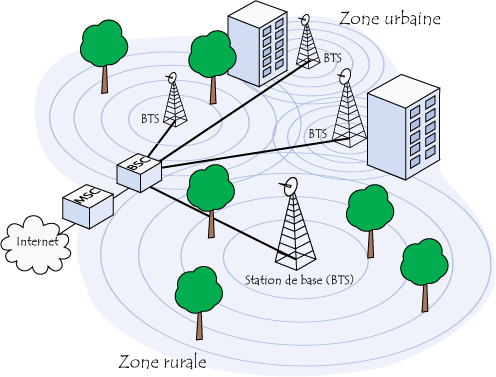
\includegraphics[width=\linewidth]{img/structure_reseau_gsm.png}
    \caption{Structure du réseau GSM}
\end{figure}

Le réseau est composé de nombreux BTS (Base Transceiver System : antennes et équipement qui
couvrent une cellule) qui sont connectés entre eux à travers des BSC
(Base Station Controller) eux-mêmes reliés à des MSC (Mobile Switching
Center) qui transmettent à travers Internet les appels aux réseaux fixes
et GSM concurrents. \newline

\subsection{Exercices}

Formules utiles :

\begin{itemize}
\item[$P_{T_i}$] Puissance émetteur isotrope équivalente
\item[$P_{R_i}$] Puissance récepteur isotrope équivalente
\item[$P_T$] Puissance émetteur
\item[$G_T$] Gain émetteur
\item[$P_R$] Puissance récepteur
\item[$G_R$] Gain Récepteur
\item[$L_c$] Pertes dans le cable
\item[$L_{FS}$] Perte dans l'air
\item[$D$] portée (durant le cours c'est $r$, le rayon isotrope
\item[$A$] Air effective de l'antenne
\end{itemize}

$$P_{T_i} = \frac{P_TG_T}{L_c}$$
$$L_{FS} = \left(\frac{4\pi D}{\lambda}\right)^2$$
Dans la formule suivante, si il s'agit d'une parabole on doit multiplier les pertes au dénominateur par $\theta$ (les pertes causé par la pluie, la moisisure, les gaz, ...).
$$P_R = P_{T_i}G_R \left(\frac{\lambda}{4\pi D}\right)^2=\frac{P_{T_i}G_R}{L_{FS}}$$
$$P_R = \frac{A}{4\pi D^2}P_TG_T$$
$$P_R = P_{R_i}G_R$$

\subsubsection*{Si ma ligne atténue le signal d'un facteur de 10000 en puissance sur 1km,
quelle est le facteur d'atténuation en dB/m? }

Un facteur de $10000$ par kilomètre correspond à un facteur de 10 en
mètres.

\[ 10log(10) = 10[dB\div m] \]

\subsubsection*{Si j'utilise un récepteur super hétérodyne avec une fréquence intermédiaire
  de 20kHz, quelle doit être la fréquence de l'oscillateur local pour recevoir
une station à 100kHz? Quelle est la fréquence image?}



\subsubsection*{Illustrez la compression par Lempe-Ziv de la séquence suivante :
  ``O1OO11OOOOO11O11O11O'', à partir du $67^{ieme}$ bit.}


\newpage
  \begin{thebibliography}{1}
\bibitem{AttWiki} http://fr.wikipedia.org/wiki/Atténuation
\bibitem{BruitWiki} http://fr.wikipedia.org/wiki/Bruit\#Usages\_sp.C3.A9cialis.C3.A9s
\bibitem{DistWiki} http://fr.wikipedia.org/wiki/Distorsion\_\%28audio\%29
\bibitem{B31} G. Pinson, {\em Modèle à constante répartie d'une ligne de transmission}, ISBN 2-9520781-0-6, http://www.syscope.net/elec/B31.pdf
\bibitem{Propagation} P.G. Fontolliet, {\em Traité d'Electricité}, Volume XVIII, Ecole polytechnique fédéral de Lausanne, pp 72-73
\bibitem{Biwi} http://fr.wikipedia.org/wiki/Ligne\_bifilaire
\bibitem{Diwi} http://fr.wikipedia.org/wiki/Diaphonie
\bibitem{Coax} http://www.commentcamarche.net/contents/1128-transmission-de-donnees-le-cablage
\bibitem{Fopt} http://fr.wikipedia.org/wiki/Fibre\_optique
\bibitem{Dmod} http://fr.wikipedia.org/wiki/Dispersion\_intermodale
\bibitem{Transducteur} http://fr.wikipedia.org/wiki/Transducteur
\bibitem{Ion}http://fr.wikipedia.org/wiki/Propagation\_ionosph\%C3\%A9rique
\bibitem{WikiAntenne}http://fr.wikipedia.org/wiki/Antenne\_radio\%C3\%A9lectrique
\bibitem{WikiTEM}http://fr.wikiversity.org/wiki/Ondes\_\%C3\%A9lectromagn\%C3\%A9tiques\_guid\%C3\%A9es/G\%C3\%A9n\%C3\%A9ralit\%C3\%A9s
\bibitem{deptinfo}http://deptinfo.cnam.fr/Enseignement/Memoires/LUSTEAU.Franck/Pages/Notions\_de\_base.htm
\bibitem{ulg}http://www2.ulg.ac.be/telecom/teaching/notes/total0/elen036/node75\_mn.html
\bibitem{rennes}http://perso.univ-rennes1.fr/gilles.choisy/trame/modulation.htm
\bibitem{tafro}http://www.ta-formation.com/acrobat-modules/fm.pdf
\bibitem{sonelec}http://www.sonelec-musique.com/electronique\_bases\_diffusion\_fm\_preac\_desac.html
\bibitem{sh}http://fr.wikipedia.org/wiki/R\%C3\%A9cepteur\_superh\%C3\%A9t\%C3\%A9rodyne
\bibitem{resume}{\em LELEC1930 : Introduction aux télécommunications: résumé général}, page 6
\bibitem{sh2}http://fr.wikipedia.org/wiki/D\%C3\%A9tection\_h\%C3\%A9t\%C3\%A9rodyne
\bibitem{pilot}http://en.wikipedia.org/wiki/Pilot\_signal
\bibitem{SECAM}http://fr.wikipedia.org/wiki/S\%C3\%89CAM
\bibitem{radioelec}http://www.radio-electronics.com/info/cellulartelecomms/gsm\_technical/power-control-classes-amplifier.php
\bibitem{ccm}http://www.commentcamarche.net/contents/1120-edge-enhanced-data-rates-for-gsm-evolution
\bibitem{dct}http://lmrs.univ-rouen.fr/Vulgarisation/JPEG/jpeg-DCT.html
\bibitem{dct2}http://fr.wikipedia.org/wiki/JPEG
\bibitem{des}http://en.kioskea.net/contents/134-introduction-to-encryption-with-des
\bibitem{ccmssl}http://www.commentcamarche.net/contents/215-ssl-secure-sockets-layers
\bibitem{hamming}http://michael.dipperstein.com/hamming/
\bibitem{dsl}http://fr.wikipedia.org/wiki/Digital\_Subscriber\_Line
\bibitem{isdn}http://fr.wikipedia.org/wiki/R\%C3\%A9seau\_num\%C3\%A9rique\_\%C3\%A0\_int\%C3\%A9gration\_de\_services
\bibitem{vdsl}http://fr.wikipedia.org/wiki/Very\_High\_Bitrate\_Digital\_Subscriber\_Line
\end{thebibliography}

\end{document}
